\documentclass[utf8]{FrontiersinVancouver}

\usepackage{url,hyperref,lineno,microtype,subcaption}
\usepackage[onehalfspacing]{setspace}
\usepackage{graphicx}
\usepackage{amsmath}
\usepackage{booktabs}
\usepackage{array}
\usepackage{tabularx}

\linenumbers
\setcitestyle{square,numbers}
\emergencystretch=2em

\def\keyFont{\fontsize{8}{11}\helveticabold}
\def\firstAuthorLast{Jin {et~al.}}
\def\Authors{Zhi Jin\,$^{1,*}$, Hua Sun\,$^{1}$, Yiting Zhou\,$^{2}$ and Shuang Wu\,$^{3,*}$}
\def\Address{$^{1}$College of Information Engineering, Changsha Medical University, Changsha 410219, Hunan, China \\
$^{2}$School of Computer Science and Technology, Changsha University of Science and Technology, Changsha, Hunan, China \\
$^{3}$The Affiliated Changsha Central Hospital, Hengyang Medical School, University of South China, Changsha 410004, Hunan, China}
\def\corrAuthor{Zhi Jin and Shuang Wu}
\def\corrEmail{\nolinkurl{jinzhi1@csmu.edu.cn}; \nolinkurl{2018051139@usc.edu.cn}}

\begin{document}
\onecolumn
\firstpage{1}

\title[GERI-NutriRisk-ICU]{GERI-NutriRisk-ICU: an APACHE-contextualized, hospital-robust, and nutrition-aware domain-updated framework for mortality risk stratification in older ICU patients}

\author[\firstAuthorLast]{\Authors}
\address{}
\correspondance{}
\extraAuth{Author email addresses: Hua Sun, \nolinkurl{mssun@csmu.edu.cn}; Yiting Zhou, \nolinkurl{zyt_csust@csust.edu.com}.}

\maketitle

\begin{abstract}
\section{}
\textbf{Objective:} Older intensive care unit (ICU) patients face intertwined nutrition risk, metabolic instability, and acute physiologic severity. A framework integrating MIMIC-IV/eICU-CRD external validation, APACHE-IV/IVa benchmarking, calibration, and explainable machine learning can clarify the measurable role of nutrition-related variables in this setting. We developed GERI-NutriRisk-ICU for early, nutrition-aware mortality risk stratification in older ICU patients.
\textbf{Methods:} This retrospective multicohort study included ICU stays from patients aged 65 years or older in MIMIC-IV and eICU-CRD. MIMIC-IV supported model development and source-domain testing; eICU-CRD supported external validation, prespecified local domain updating, disjoint Platt calibration, and held-out evaluation. The endpoint was in-hospital mortality, harmonized from discharge-status fields. The final schema contained 83 cross-database predictors covering demographics, body mass index, nutrition-support indicators, nutrition/metabolic laboratories, vital signs, blood gas/perfusion variables, organ support, neurologic severity, urine output, and ICU/admission context. Analyses included tabular-learning comparators, nutrition-feature ablations, APACHE-IV/IVa same-subset comparisons, explainability, decision-curve analysis, and hospital-cluster robustness.
\textbf{Results:} The cohorts contained 33,671 MIMIC-IV stays and 71,861 eICU-CRD stays. Source-only transport gained discrimination after feature expansion but remained below APACHE-IV/IVa on the APACHE-available eICU subset. The locked domain-updated head achieved held-out eICU AUROC 0.872, Brier score 0.073, and expected calibration error 0.004 in 57,488 stays. In the APACHE-IVa-available held-out subset, GERI-NutriRisk-ICU achieved AUROC 0.871 versus 0.850 for APACHE-IVa, with paired AUROC difference 0.0209 (95\% CI 0.0158--0.0260) and lower Brier score (0.074 vs. 0.082). Hospital-cluster bootstrap confirmed this advantage (mean AUROC difference 0.021; 95\% cluster CI 0.015--0.028). Removing the full nutrition construct reduced domain-updated AUROC by 0.0049 (95\% CI 0.0029--0.0071), and removing nutrition/metabolic laboratories reduced AUROC by 0.0059 (95\% CI 0.0041--0.0077).
\textbf{Conclusion:} GERI-NutriRisk-ICU delivered calibrated, APACHE-contextualized, hospital-robust, and nutrition-aware mortality risk stratification for older ICU patients. The results position nutrition and metabolic variables as modest but reproducible contributors within integrated ICU severity modeling and support prospective evaluation of nutrition-aware risk surveillance.

\tiny
\keyFont{\section{Keywords:} geriatric intensive care, nutrition risk, mortality prediction, MIMIC-IV, eICU-CRD, APACHE-IV, calibration, explainable machine learning}
\end{abstract}

\section{Introduction}

Older adults admitted to intensive care units (ICUs) enter critical illness with a distinctive combination of reduced physiologic reserve, pre-existing vulnerability, acute inflammation, metabolic stress, and rapidly changing nutrition-support needs. Contemporary ICU nutrition guidance therefore treats nutrition assessment as an early component of critical-care decision-making rather than a late adjunct after stabilization \citep{Singer2023ESPENPractical,Compher2022ASPEN,deMan2024ICUNutrition}. In this population, nutrition-related information is clinically meaningful because it reflects body composition, protein-energy reserve, inflammatory catabolism, organ dysfunction, and treatment processes that evolve during the first ICU day.

The geriatric context sharpens this problem. Frailty, sarcopenia, multimorbidity, and baseline functional limitation modify the relationship between an acute physiologic insult and hospital outcome, while malnutrition and nutrition risk remain difficult to distinguish from the severity of the critical illness itself \citep{Compher2025GLIMCriticalIllness,Moisi2024Frailty,Inaba2023Frailty}. A risk model for older ICU patients must therefore avoid a narrow interpretation of albumin, body mass index, feeding records, or metabolic laboratories as isolated nutrition markers. These variables are better understood as part of an integrated vulnerability phenotype that combines nutritional reserve, metabolic response, and acute organ failure.

Existing clinical tools address different parts of this phenotype but leave an important gap for nutrition-aware electronic risk stratification. The NUTRIC framework and related nutrition indices were designed to identify critically ill patients at higher nutrition risk, whereas APACHE-IV/IVa provides a mature ICU mortality benchmark built around global acute physiology and chronic health evaluation \citep{Heyland2011NUTRIC,Peng2023GNRI,Zimmerman2006ApacheIV}. Recent machine-learning work has improved automated nutrition-risk screening from electronic health records, but much of this evidence remains focused on single-database development, internally held-out validation, or nutrition diagnosis rather than APACHE-contextualized mortality prediction across critical-care databases \citep{Zhang2026ENUTRIC,Cao2026NIM}.

Public critical-care databases make this question reproducible, but they also expose the central weakness of many computational clinical studies. MIMIC-IV and eICU-CRD differ in hospital composition, documentation practices, variable availability, measurement frequency, and care-process coding \citep{Johnson2023MIMICIV,Pollard2018EICU}. A model that performs well inside one database can lose discrimination or probability calibration after transport because it has learned local missingness patterns, thresholds for laboratory ordering, or site-specific treatment workflows rather than transportable physiology.

For that reason, the evidentiary standard for a nutrition-facing ICU prediction framework should extend beyond reporting a high AUROC. Current prediction-model guidance emphasizes external validation, transparent reporting, risk-of-bias assessment, calibration, and the distinction between model development, model updating, and independent evaluation \citep{Collins2024EvalPart1,Riley2024EvalPart2,Collins2024TRIPODAI}. The same logic is especially important for artificial-intelligence and machine-learning models, where flexible algorithms can amplify leakage, post hoc model selection, and optimistic interpretation if comparator choice, calibration, and held-out validation are not prespecified \citep{Moons2025PROBASTAI,VanCalster2023NoValidated,VanCalster2019Calibration}.

Recent ICU machine-learning studies increasingly use multicohort designs, interpretable feature attribution, and clinical utility analyses, showing that routinely measured physiologic and laboratory variables can support externally evaluated risk stratification \citep{Zhang2025IBD,Liu2026TabPFN,Huynh2026PAR}. However, this literature still leaves three unresolved requirements for older ICU nutrition-risk research. First, nutrition and metabolic variables need to be tested for incremental value inside a full acute-severity framework rather than presented as standalone associations. Second, performance must be evaluated against a credible ICU severity comparator on the same records. Third, model claims should combine discrimination, calibration, clinical utility, explainability, and hospital-level robustness rather than relying on a single aggregate metric \citep{Vickers2006DCA,Ghassemi2021XAI}.

We developed GERI-NutriRisk-ICU to address these requirements. The framework harmonizes first-day demographics, body mass index, nutrition-support indicators, nutrition/metabolic laboratories, vital signs, blood gas and perfusion variables, organ support, neurologic severity, urine output, and ICU/admission context across MIMIC-IV and eICU-CRD. Methodologically, it combines a standardized logistic anchor for coefficient-level interpretation, a bounded tabular-learning comparator queue, a locked LightGBM performance head, prespecified local target-domain updating, disjoint Platt recalibration, and held-out eICU evaluation \citep{Chen2016XGBoost,Ke2017LightGBM}.

The contribution of this study is threefold. First, we establish an auditable MIMIC-IV to eICU-CRD framework for early mortality-risk stratification in older ICU patients, separating source-only transport from target-domain updating and disjoint calibration. Second, we benchmark the locked model against APACHE-IV/IVa predictions on the identical held-out eICU subset, directly testing whether the updated framework adds predictive resolution beyond a mature ICU severity standard. Third, we quantify the incremental value of nutrition-related feature domains and connect model behavior to grouped permutation importance, decision-curve analysis, and hospital-cluster robustness. In the final held-out eICU evaluation, GERI-NutriRisk-ICU achieved AUROC 0.872, Brier score 0.073, and expected calibration error 0.004; on the APACHE-IVa-available subset, it exceeded APACHE-IVa by 0.0209 AUROC with a lower Brier score. Figure~\ref{fig:workflow} summarizes the full study design.

\begin{figure}[htbp]
\centering
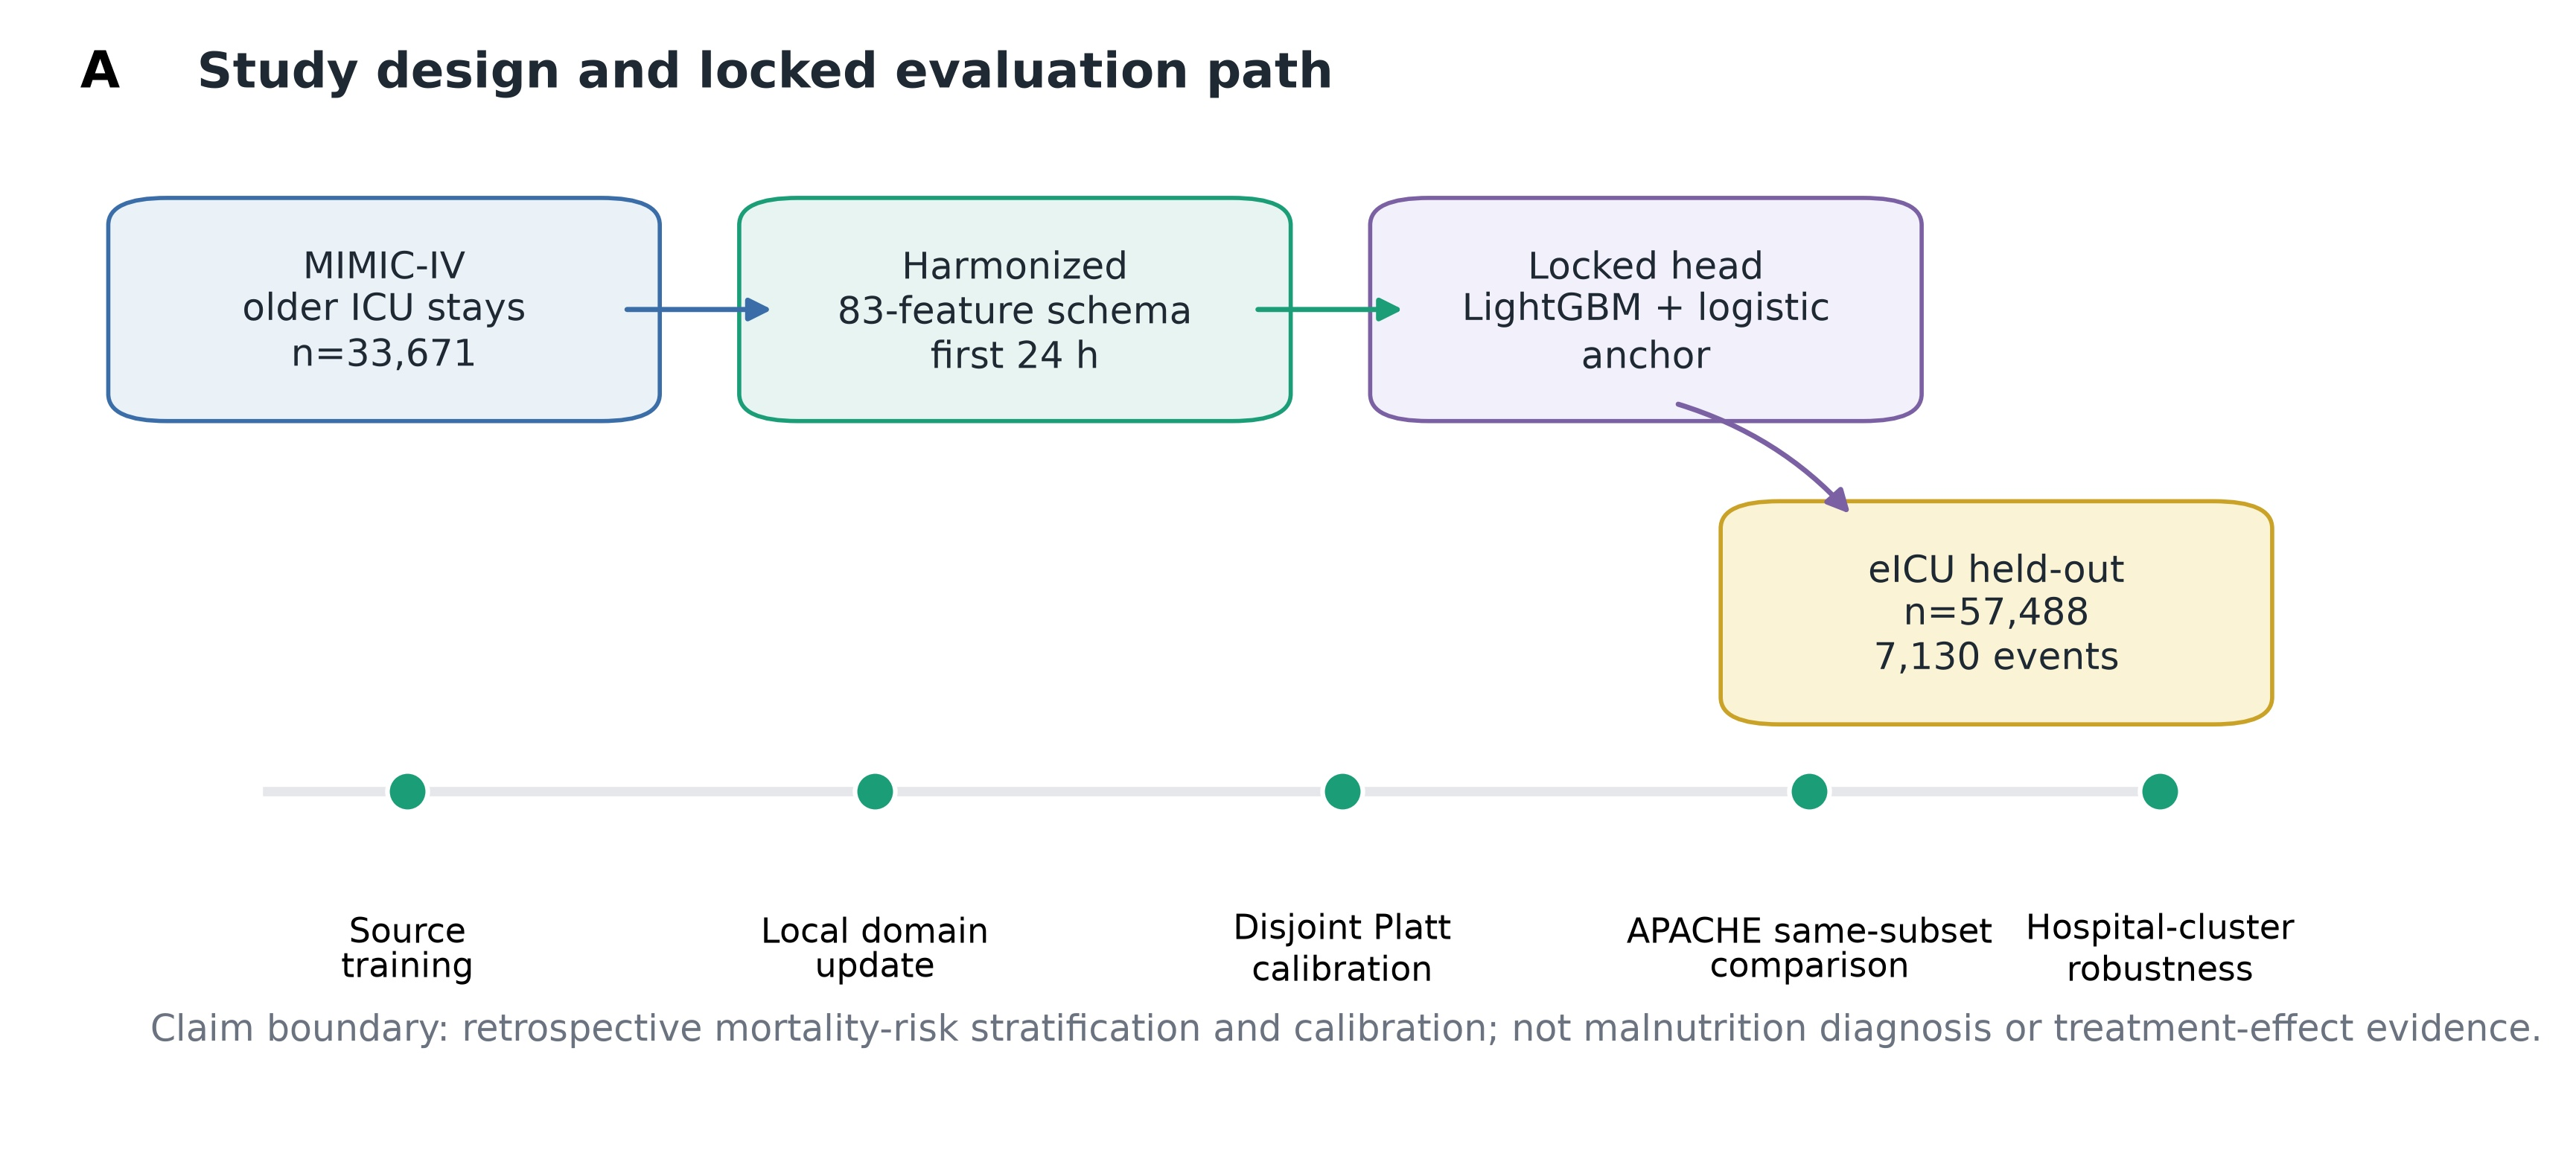
\includegraphics[width=0.92\textwidth]{../../figures/main_fig1_workflow.jpg}
\caption{Development, feature harmonization, modeling, domain updating, calibration, and held-out evaluation workflow for GERI-NutriRisk-ICU. MIMIC-IV v3.1 was used as the source-domain development cohort and eICU-CRD as the target-domain validation, local-update, calibration, and held-out evaluation cohort. APACHE-IV/IVa predictions were used only as same-subset clinical comparators.}
\label{fig:workflow}
\end{figure}

\section{Methods}

\subsection{Study Design and Data Sources}
This study was designed as a retrospective multicohort prediction-model study with a source-domain database, an external target-domain database, and a prespecified target-domain update and calibration path. MIMIC-IV v3.1 served as the source database for feature development, model fitting, and internal testing, whereas eICU-CRD v2.0 served as the multicenter target database for external validation, local updating, calibration, and held-out evaluation \citep{PhysioNetMIMICIV31,PhysioNetEICU20,Johnson2023MIMICIV,Pollard2018EICU}. The clinical question was framed as early mortality-risk stratification for older ICU patients in whom nutritional vulnerability, metabolic instability, and acute physiologic severity coexist. The intended prediction time was the first day of ICU care, before hospital outcome ascertainment.

Eligible records were ICU stays among patients aged 65 years or older. We used ICU stays rather than unique patients as the modeling unit because the available exposures, physiologic summaries, organ-support indicators, and discharge outcomes are attached to a specific critical-care encounter. The source-domain sample is denoted by $\mathcal{D}_{S}=\{(\mathbf{x}_{i}^{S},y_{i}^{S})\}_{i=1}^{n_{S}}$, and the target-domain sample is denoted by $\mathcal{D}_{T}=\{(\mathbf{x}_{i}^{T},y_{i}^{T})\}_{i=1}^{n_{T}}$. Patient-level records remained on the secured analysis server; local manuscript assets contain aggregate tables, figure source data, code, logs, and non-identifying summaries.

\subsection{Cohort Definition and Outcome}
The MIMIC-IV cohort contained 33,671 ICU stays with 4,659 in-hospital deaths, and the eICU-CRD cohort contained 71,861 ICU stays with 8,860 in-hospital deaths (Table~\ref{tab:cohort}). The endpoint was in-hospital mortality, defined from \texttt{hospital\_expire\_flag} in MIMIC-IV and \texttt{hospitaldischargestatus} coded as expired in eICU-CRD. For stay $i$, the binary outcome was encoded as
\begin{equation}
y_i =
\begin{cases}
1, & \text{if hospital discharge status indicated death before discharge},\\
0, & \text{otherwise}.
\end{cases}
\label{eq:outcome}
\end{equation}
Equation~\ref{eq:outcome} defines an auditable adverse hospital outcome that can be harmonized across both databases. The endpoint supports nutrition-aware risk stratification because it captures severe adverse prognosis in an older ICU population, while malnutrition status, nutritional adequacy, and nutrition-treatment response remain distinct constructs. This boundary is central to the study interpretation: GERI-NutriRisk-ICU estimates mortality risk in a nutrition-aware feature space rather than diagnosing a nutrition disorder.

\begin{table}[htbp]
\centering
\caption{Cohort summary.}
\label{tab:cohort}
\begin{tabular}{lrrrrrr}
\toprule
Cohort & Stays & Events & Event rate & Ventilation & Dialysis & Median GCS\\
\midrule
MIMIC-IV & 33,671 & 4,659 & 0.138 & 10,920 & 409 & 13\\
eICU-CRD & 71,861 & 8,860 & 0.123 & 14,754 & 1,620 & 15\\
\bottomrule
\end{tabular}
\end{table}

\subsection{Predictors and Framework}
Predictors were restricted to variables available during the first 24 hours after ICU admission or to baseline admission fields available before outcome ascertainment. Let $a_i$ be the ICU admission time for stay $i$ and let $W_i=[a_i,a_i+24\text{ h}]$ be the feature-observation window. For raw clinical measurements $z_{ij}(t)$ and baseline fields $\mathbf{b}_{i}$, each harmonized predictor was generated through a prespecified extraction and mapping operator,
\begin{equation}
x_{ij}=H_j\left(\{z_{ij}(t):t\in W_i\},\mathbf{b}_{i}\right),\quad j=1,\ldots,p,
\label{eq:feature_map}
\end{equation}
where $p=83$ in the locked full schema. Equation~\ref{eq:feature_map} formalizes the main leakage-control principle: the feature vector $\mathbf{x}_{i}$ can depend on early-window measurements and admission-context fields, but not on discharge status, length of stay, procedures after the baseline window, or outcome-derived quantities.

The final schema included demographics, body mass index, enteral and parenteral nutrition-support indicators, albumin, glucose, creatinine, blood urea nitrogen, sodium, bilirubin, hematocrit, white blood cell count, vital signs, blood gas/perfusion markers including lactate and PaO$_2$/FiO$_2$ ratio, coagulation and hematology, urine output, ventilation, dialysis, Glasgow Coma Scale, ICU type, and admission-source context. Missingness indicators were retained when they were clinically informative and consistently mappable:
\begin{equation}
m_{ij}=I(x_{ij}\ \text{is not observed in}\ W_i).
\label{eq:missingness}
\end{equation}
Equation~\ref{eq:missingness} treats missingness as part of the observable electronic-health-record process rather than as a post hoc nuisance term. This choice is clinically relevant in ICU data because the absence of a measurement may reflect triage, illness severity, clinical suspicion, or workflow patterns. Cross-database harmonization required each retained feature to have a documented MIMIC-IV source, an eICU-CRD source, directionally consistent clinical meaning, and explicit missingness handling.

\subsection{GERI-NutriRisk-ICU Framework}
GERI-NutriRisk-ICU separates four functions: a standardized logistic anchor for transparent interpretation, a protocolized tabular-learning benchmark, a locked LightGBM performance head, and an external-domain calibration layer. For all model families, the uncalibrated risk score was written as
\begin{equation}
\hat{p}_i=f_{\theta}(\mathbf{x}_i),\quad 0\leq \hat{p}_i\leq 1,
\label{eq:risk_model}
\end{equation}
Equation~\ref{eq:risk_model} defines the common risk-function notation used for the logistic anchor, LightGBM head, and comparator models. Here $\hat{p}_i$ is the predicted probability of the outcome in Equation~\ref{eq:outcome}. The transparent anchor used standardized predictors and a logistic link,
\begin{equation}
\hat{p}^{\mathrm{LR}}_i=\sigma\left(\beta_0+\sum_{j=1}^{p}\beta_j\tilde{x}_{ij}\right),\quad
\sigma(u)=\frac{1}{1+\exp(-u)}.
\label{eq:logistic_anchor}
\end{equation}
Equation~\ref{eq:logistic_anchor} provided coefficient-level face-validity checks and a stable reference model. The performance head used LightGBM, selected after protocolized comparison against XGBoost, CatBoost, HistGradientBoosting, random forest, ExtraTrees, multilayer perceptron, and TabNet. The comparator queue covered mature gradient-boosting families \citep{Chen2016XGBoost,Ke2017LightGBM,Prokhorenkova2018CatBoost} and a neural tabular comparator \citep{Arik2021TabNet}. LightGBM was retained because no comparator achieved a material held-out recalibrated eICU AUROC gain greater than 0.015 while preserving calibration and interpretability tradeoffs. Supplementary Material reports the full comparator queue.

The source-only model estimated $\theta$ from the MIMIC-IV development set and transported the fitted function unchanged to eICU-CRD. The domain-updated head estimated the final performance model from MIMIC-IV development data plus a prespecified eICU local-update subset. In compact form, the nested fitting objective was
\begin{equation}
\hat{\theta}_{S+T_u}=
\arg\min_{\theta}
\left[
\frac{1}{|\mathcal{D}_{S}^{\mathrm{dev}}|}
\sum_{i\in \mathcal{D}_{S}^{\mathrm{dev}}}\ell\{y_i,f_{\theta}(\mathbf{x}_i)\}
+
\lambda
\frac{1}{|\mathcal{D}_{T}^{u}|}
\sum_{i\in \mathcal{D}_{T}^{u}}\ell\{y_i,f_{\theta}(\mathbf{x}_i)\}
\right],
\label{eq:domain_update}
\end{equation}
where $\ell$ denotes binary prediction loss and $\mathcal{D}_{T}^{u}$ denotes the eICU local-update subset. Equation~\ref{eq:domain_update} clarifies the distinction between direct transport and domain-updated validation: target-domain labels were used only in the declared update subset, and evaluation used a disjoint held-out eICU subset.

\subsection{Validation and Statistical Analysis}
MIMIC-IV records were split into development and internal-test partitions using a fixed row-index rule. eICU-CRD was then partitioned into non-overlapping local-update, calibration, and held-out evaluation subsets. If $r_i$ denotes the fixed eICU row index, the nested target-domain partition was
\begin{equation}
\mathcal{D}_{T}^{u}=\{i:r_i\bmod 10=0\},\quad
\mathcal{D}_{T}^{c}=\{i:r_i\bmod 10=5\},\quad
\mathcal{D}_{T}^{h}=\{i:r_i\bmod 10\notin\{0,5\}\}.
\label{eq:eicu_split}
\end{equation}
The source-only analysis trained on MIMIC-IV and evaluated eICU without eICU model fitting except for explicitly labeled Platt recalibration. The final nested analysis used $\mathcal{D}_{T}^{u}$ for local updating, $\mathcal{D}_{T}^{c}$ for calibration, and $\mathcal{D}_{T}^{h}$ for final evaluation as specified in Equation~\ref{eq:eicu_split}. This partitioning establishes record-level separation among local updating, calibration, and held-out evaluation; hospital-level dependence was assessed separately through site-restriction analyses and hospital-cluster bootstrap.

External recalibration used a Platt layer fitted only on the calibration subset and then applied unchanged to held-out predictions:
\begin{equation}
\hat{p}^{\mathrm{cal}}_i=
\sigma\left\{\alpha+\gamma\,\operatorname{logit}(\hat{p}_i)\right\}.
\label{eq:platt}
\end{equation}
Equation~\ref{eq:platt} separates rank learning from probability-scale correction. This distinction matters because source-only transport can retain clinically useful ordering while producing miscalibrated absolute risks after the measurement, coding, and treatment-process distribution shifts from MIMIC-IV to eICU-CRD.

Discrimination was evaluated by AUROC, interpreted as the probability that a randomly selected event stay receives a higher predicted risk than a randomly selected non-event stay:
\begin{equation}
\operatorname{AUROC}=P(\hat{p}_{i:y_i=1}>\hat{p}_{j:y_j=0}).
\label{eq:auroc}
\end{equation}
Calibration was evaluated by Brier score, ECE, and calibration curves. The Brier score was defined as
\begin{equation}
\operatorname{Brier}=\frac{1}{n}\sum_{i=1}^{n}(y_i-\hat{p}^{\mathrm{cal}}_i)^2,
\label{eq:brier}
\end{equation}
and ECE with $K=10$ quantile bins was defined as
\begin{equation}
\operatorname{ECE}=\sum_{k=1}^{K}\frac{|B_k|}{n}\left|
\frac{1}{|B_k|}\sum_{i\in B_k}y_i-
\frac{1}{|B_k|}\sum_{i\in B_k}\hat{p}^{\mathrm{cal}}_i
\right|.
\label{eq:ece}
\end{equation}
Equations~\ref{eq:auroc}, \ref{eq:brier}, and \ref{eq:ece} were reported together because a model that ranks patients well can still be poorly calibrated for threshold-based risk communication.

APACHE-IV and APACHE-IVa predicted hospital mortality were evaluated only as same-subset comparators and were never used as model inputs. On the APACHE-available held-out subset, paired performance differences were calculated as
\begin{equation}
\Delta_{\mathrm{AUC}}=\operatorname{AUROC}(\hat{p}^{\mathrm{GERI}})-\operatorname{AUROC}(\hat{p}^{\mathrm{APACHE}}),\quad
\Delta_{\mathrm{Brier}}=\operatorname{Brier}(\hat{p}^{\mathrm{GERI}})-\operatorname{Brier}(\hat{p}^{\mathrm{APACHE}}).
\label{eq:paired_delta}
\end{equation}
Equation~\ref{eq:paired_delta} ensures that clinical-benchmark comparisons use identical patient records. Nutrition-feature incremental value used the same paired full-minus-reduced logic, with positive $\Delta_{\mathrm{AUC}}$ and negative $\Delta_{\mathrm{Brier}}$ favoring the full nutrition-aware schema. Feature-domain explainability used LightGBM gain and grouped permutation importance on $\mathcal{D}_{T}^{h}$; for feature group $G$, the grouped AUROC decrease was
\begin{equation}
\Delta_{\mathrm{perm}}(G)=\operatorname{AUROC}(\hat{p})-\operatorname{AUROC}(\hat{p}^{\pi(G)}),
\label{eq:permutation}
\end{equation}
Equation~\ref{eq:permutation} quantifies the held-out discrimination loss attributable to a feature domain, where $\pi(G)$ denotes permutation of the features in group $G$ while other predictors remain unchanged. Clinical utility was summarized with decision-curve net benefit,
\begin{equation}
\operatorname{NB}(p_t)=\frac{\operatorname{TP}(p_t)}{n}-\frac{\operatorname{FP}(p_t)}{n}\frac{p_t}{1-p_t},
\label{eq:net_benefit}
\end{equation}
as shown in Equation~\ref{eq:net_benefit} across prespecified threshold probabilities $p_t$ \citep{Vickers2006DCA}. Hospital robustness was assessed by excluding the ten largest eICU hospitals, restricting to hospitals with at least 100 or 200 held-out stays, and bootstrapping hospitals as clusters. All final lock experiments were rerun on the remote analysis server, and the server-side evidence manifest recorded v7--v16 result hashes and logs.

\section{Results}

The results are organized as a stepwise validation chain. We begin with feature-family development and source-only transport to identify what transfers across databases, then evaluate recalibration, clinical utility, subgroup behavior, and model-class choice. The final analyses report the locked domain-updated framework, benchmark it against APACHE-IV/IVa on identical eICU records, quantify nutrition-feature incremental value, and test interpretability and hospital-level robustness.

\subsection{Feature-Family Ablation}
The feature-family ablation established the first layer of the evidence chain: cross-database mortality stratification required information beyond demographic and nutrition-support descriptors. Moving from the V0 demographic/BMI/nutrition-support schema to laboratory variables increased eICU AUROC from 0.575 to 0.643, and adding vital signs further increased AUROC to 0.666. The largest external jump occurred when general severity variables were introduced, with the severity-only baseline reaching AUROC 0.722 and the complete early GERI-NutriRisk-ICU schema reaching AUROC 0.727 (Figure~\ref{fig:ablation}, Table~\ref{tab:ablation}). This pattern indicates that early ICU mortality risk is organized around a broad physiologic vulnerability signal. Nutrition-related variables contributed to this signal most plausibly as part of the same vulnerability context, while organ support, neurologic status, and acute physiologic derangement supplied much of the transportable discrimination.

\begin{figure}[htbp]
\centering
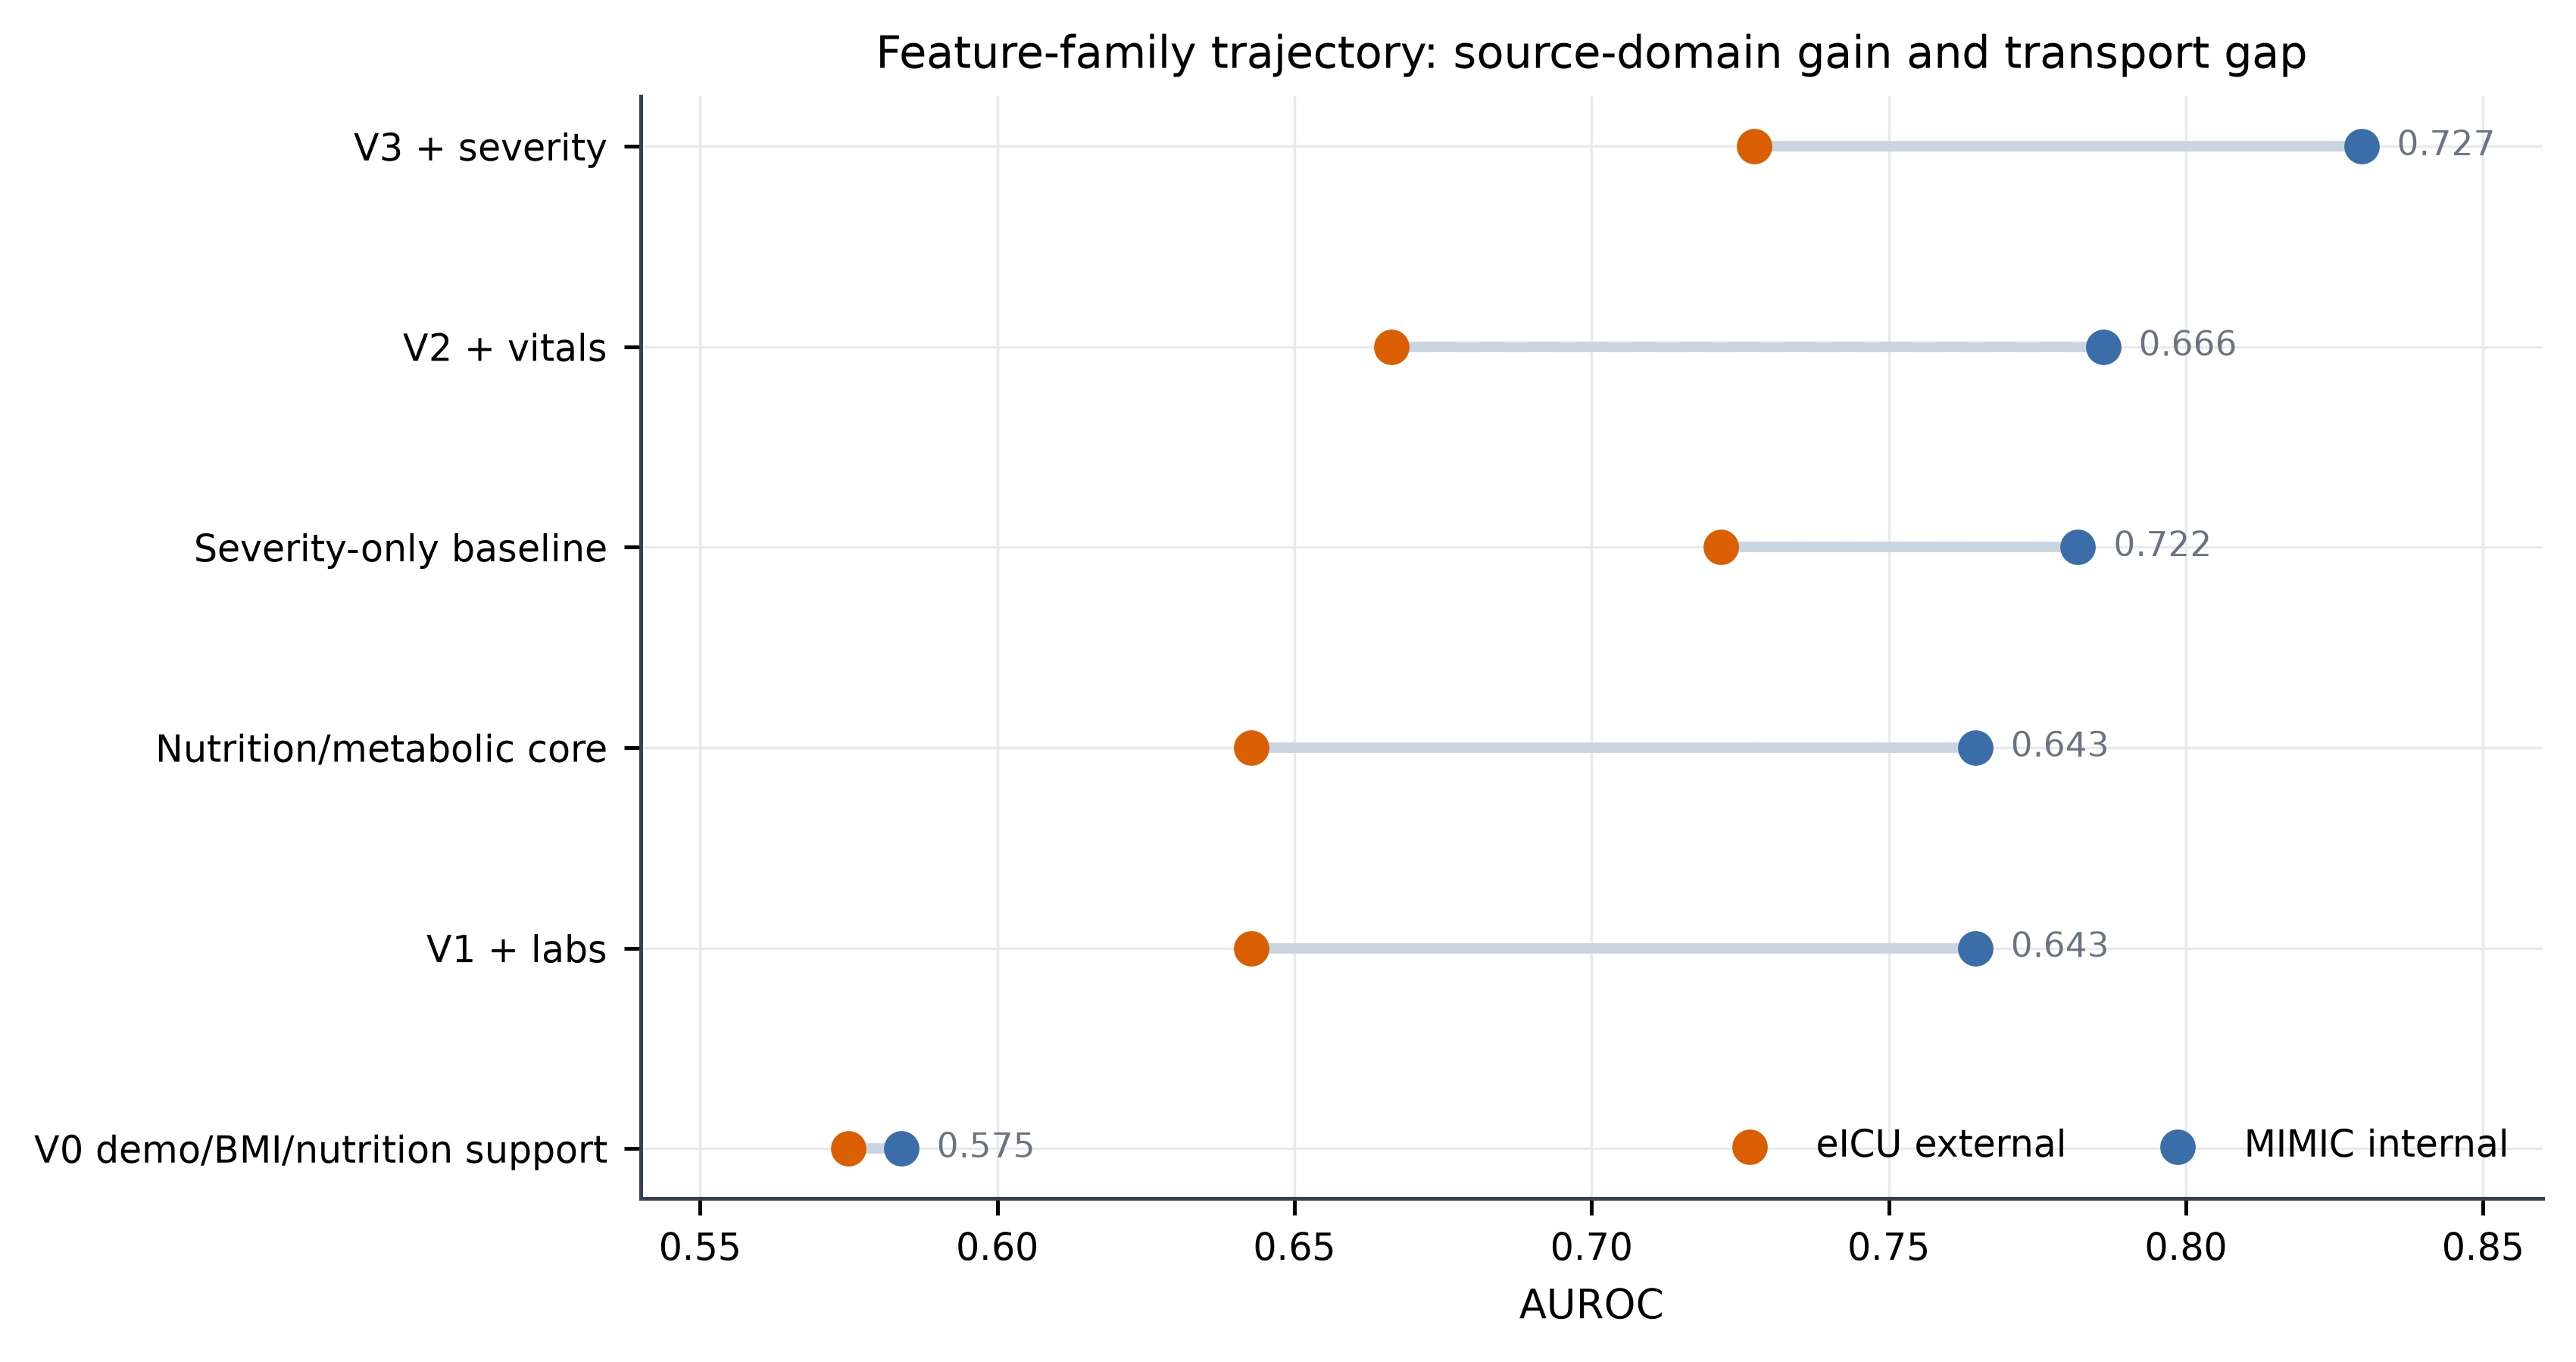
\includegraphics[width=0.82\textwidth]{../../figures/main_fig2_feature_ablation.jpg}
\caption{Feature-family development trajectory across MIMIC-IV internal testing and eICU-CRD external validation before the final domain-update lock.}
\label{fig:ablation}
\end{figure}

\begin{table}[htbp]
\centering
\caption{Feature-family ablation in the GERI-NutriRisk-ICU development trajectory. Bold values indicate the best value in each displayed metric column; lower Brier score is better.}
\label{tab:ablation}
\resizebox{\textwidth}{!}{%
\begin{tabular}{lrrrr}
\toprule
Feature schema or model & MIMIC AUROC & MIMIC Brier & eICU AUROC & eICU Brier\\
\midrule
V0 demographics/BMI/nutrition support & 0.584 & 0.119 & 0.575 & \textbf{0.108}\\
V1 plus laboratories & 0.765 & 0.105 & 0.643 & 0.137\\
V2 plus vitals & 0.786 & 0.098 & 0.666 & 0.221\\
Nutrition/metabolic core & 0.765 & 0.105 & 0.643 & 0.137\\
Severity-only baseline & 0.782 & 0.098 & 0.722 & 0.119\\
GERI-NutriRisk-ICU & \textbf{0.830} & \textbf{0.090} & \textbf{0.727} & 0.155\\
\bottomrule
\end{tabular}}
\end{table}

\subsection{Source-Only Nutrition-Construct Sensitivity}
The prespecified nutrition-construct sensitivity analysis clarified how nutrition-related information behaved before local domain updating. In source-only MIMIC-to-eICU transport, the complete V3 schema exceeded the non-nutrition clinical baseline by 0.0056 AUROC (95\% CI 0.0020--0.0090), while models that removed nutrition/metabolic laboratories or all nutrition-construct variables showed better raw calibration metrics in the external cohort (Table~\ref{tab:nutrition_increment}). This result separates two concepts that are often conflated in nutrition-risk modeling. Nutrition-related measurements carry clinically meaningful information within a larger critical-illness phenotype, and their coefficients and missingness patterns require target-database adaptation before they become stable external performance contributors. The finding therefore motivated the later domain-updated analysis as the primary test of nutrition-feature increment.

\begin{table}[htbp]
\centering
\caption{Source-only nutrition-construct sensitivity analysis for GERI-NutriRisk-ICU in eICU-CRD. Bold values indicate the best value among model rows; lower Brier score and ECE are better.}
\label{tab:nutrition_increment}
\resizebox{\textwidth}{!}{%
\begin{tabular}{lrrr}
\toprule
Model or contrast & eICU AUROC & eICU Brier & eICU ECE\\
\midrule
Full V3 & 0.727 & 0.155 & 0.180\\
Without nutrition support & 0.726 & 0.151 & 0.170\\
Without nutrition/metabolic laboratories & \textbf{0.732} & 0.118 & 0.110\\
Without all nutrition-construct variables & 0.729 & \textbf{0.114} & \textbf{0.098}\\
Non-nutrition clinical baseline & 0.722 & 0.119 & 0.107\\
Nutrition/metabolic core & 0.643 & 0.137 & 0.137\\
Full V3 minus non-nutrition clinical baseline & 0.0056 (0.0020--0.0090) & 0.0364 (0.0355--0.0374) & 0.0726 (0.0716--0.0737)\\
Full V3 minus without nutrition/metabolic laboratories & -0.0050 (-0.0084 to -0.0020) & 0.0373 (0.0365--0.0383) & 0.0697 (0.0688--0.0707)\\
\bottomrule
\end{tabular}}
\end{table}

\subsection{Primary Source-Only Performance and External Recalibration}
The source-only model showed strong internal discrimination and a clear external calibration shift. In the MIMIC-IV internal test set, GERI-NutriRisk-ICU achieved AUROC 0.830 (95\% CI 0.815--0.843), Brier score 0.090 (0.085--0.095), and ECE 0.015 (0.011--0.023). When transported unchanged to the full eICU cohort, discrimination decreased to AUROC 0.727 (0.722--0.733), and absolute risk calibration deteriorated, with Brier score 0.155 (0.153--0.156) and ECE 0.180 (0.177--0.182). Platt recalibration largely corrected the probability scale while preserving ranking performance: held-out eICU AUROC was 0.728 (0.722--0.735), Brier score improved to 0.099 (0.097--0.101), and ECE improved to 0.009 (0.008--0.012) (Table~\ref{tab:primary}). Figure~\ref{fig:calibration} shows calibration drift with retained risk ordering after source-domain transport; the corresponding ROC curve is shown in Supplementary Figure S1.

\begin{figure}[htbp]
\centering
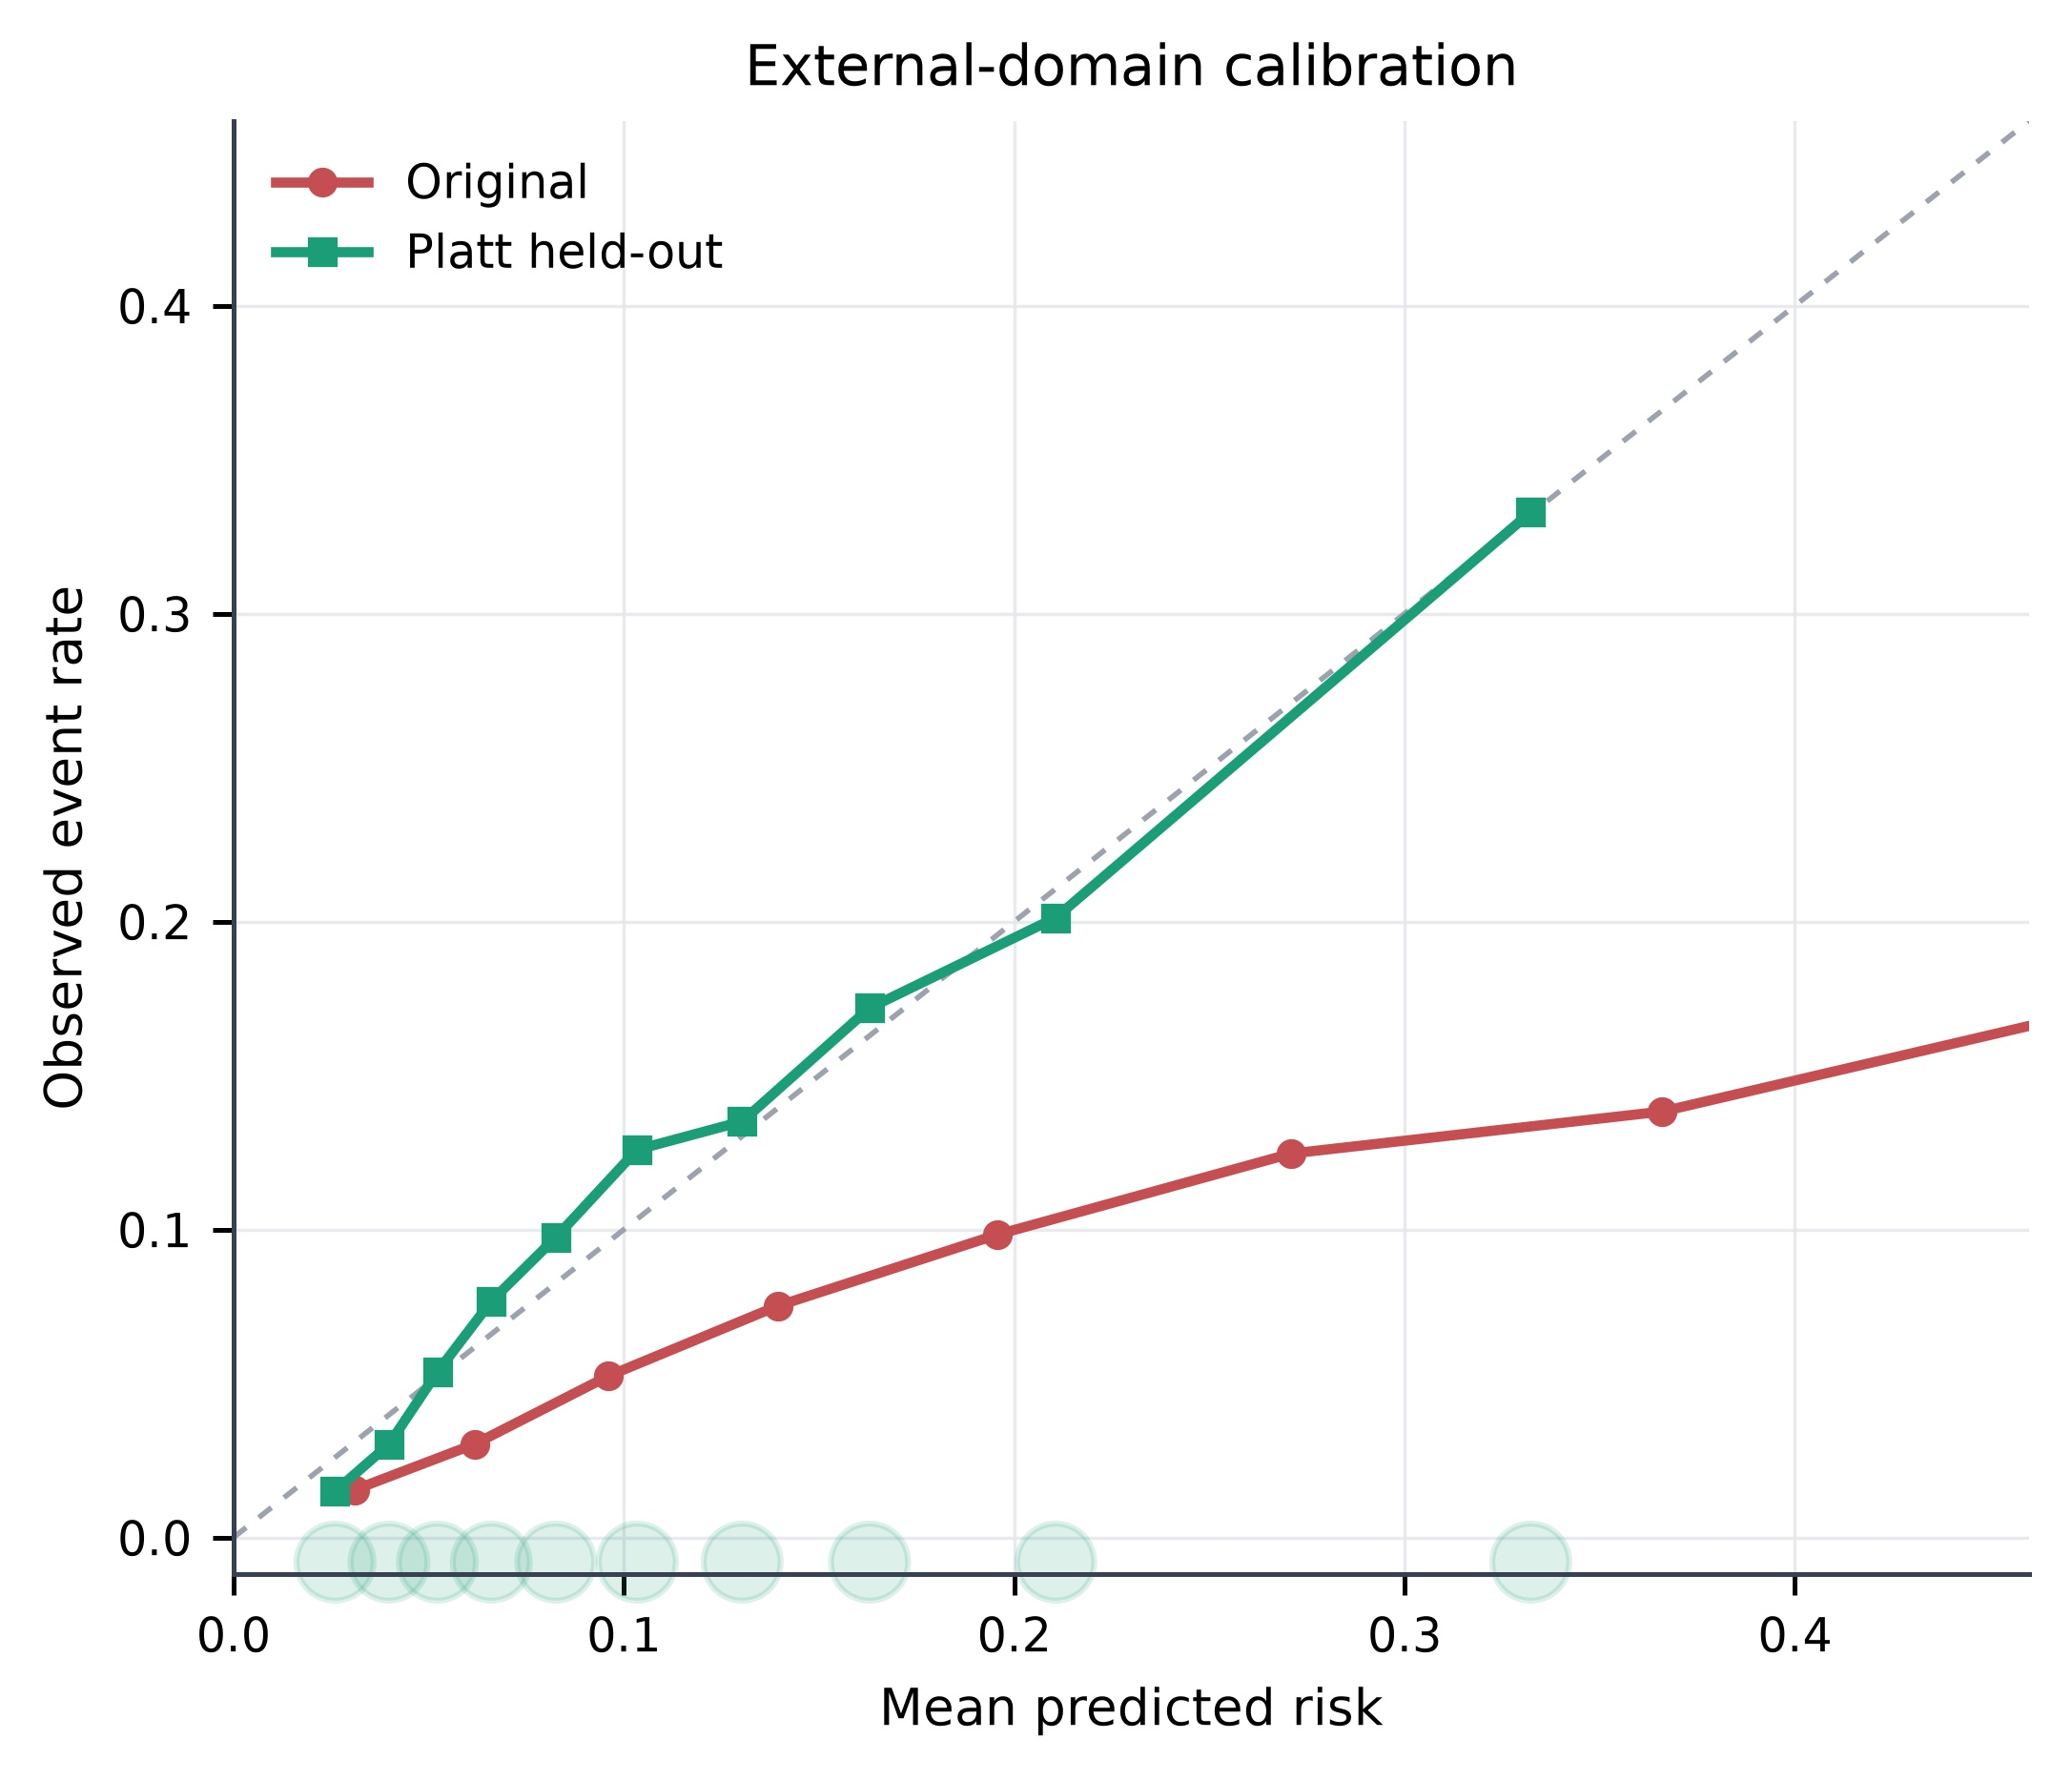
\includegraphics[width=0.70\textwidth]{../../figures/main_fig3_calibration.jpg}
\caption{External-domain calibration before and after Platt recalibration in the source-only development trajectory.}
\label{fig:calibration}
\end{figure}

\begin{table}[htbp]
\centering
\caption{Primary model performance with bootstrap confidence intervals.}
\label{tab:primary}
\resizebox{\textwidth}{!}{%
\begin{tabular}{lrrlll}
\toprule
Evaluation set & N & Events & AUROC & Brier & ECE\\
\midrule
MIMIC-IV internal test & 6,735 & 946 & 0.830 (0.815--0.843) & 0.090 (0.085--0.095) & 0.015 (0.011--0.023)\\
Full eICU external validation & 71,861 & 8,860 & 0.727 (0.722--0.733) & 0.155 (0.153--0.156) & 0.180 (0.177--0.182)\\
Held-out eICU after recalibration & 57,488 & 7,130 & 0.728 (0.722--0.735) & 0.099 (0.097--0.101) & 0.009 (0.008--0.012)\\
\bottomrule
\end{tabular}}
\end{table}

\subsection{Clinical Utility, Subgroups, and Transparent Interpretation}
Decision-curve analysis translated the calibration result into threshold-level utility. The source-only trajectory showed positive net benefit across low-to-moderate risk thresholds, and recalibration smoothed the threshold profile by aligning predicted probabilities with observed risk (Supplementary Figure S2). Subgroup analyses provided a second check on external behavior. AUROC was similar by sex, higher among ventilated patients, and lower in the oldest age group, where competing frailty burden and outcome heterogeneity likely make discrimination harder. The albumin-available subgroup had higher AUROC than the albumin-missing subgroup (0.785 vs. 0.704), suggesting that richer nutrition/metabolic measurement captured additional illness and vulnerability structure rather than merely adding an isolated laboratory marker (Table~\ref{tab:subgroup}). Standardized coefficients from the transparent anchor were clinically coherent: lower Glasgow Coma Scale and urine output, higher respiratory rate and blood urea nitrogen, older age, and higher glucose moved risk in expected directions (Supplementary Figure S3). These coefficient patterns support face-valid interpretation of the fitted risk score.

\begin{table}[htbp]
\centering
\caption{Selected eICU subgroup performance for the source-only transparent logistic anchor.}
\label{tab:subgroup}
\resizebox{\textwidth}{!}{%
\begin{tabular}{llrrrr}
\toprule
Domain & Subgroup & N & Events & AUROC & Brier\\
\midrule
Sex & Female/other & 34,780 & 4,330 & 0.723 & 0.163\\
Sex & Male & 37,081 & 4,530 & 0.733 & 0.147\\
Age & 65--74 & 31,322 & 3,114 & 0.737 & 0.129\\
Age & 75--84 & 26,004 & 3,391 & 0.717 & 0.163\\
Age & 85+ & 14,535 & 2,355 & 0.702 & 0.196\\
Albumin & Missing & 49,861 & 5,209 & 0.704 & 0.165\\
Albumin & Available & 22,000 & 3,651 & 0.785 & 0.133\\
Ventilation & No & 57,107 & 4,749 & 0.720 & 0.151\\
Ventilation & Yes & 14,754 & 4,111 & 0.754 & 0.171\\
Enteral nutrition & No & 63,935 & 7,580 & 0.727 & 0.151\\
Enteral nutrition & Yes & 7,926 & 1,280 & 0.716 & 0.185\\
\bottomrule
\end{tabular}}
\end{table}

\subsection{Split Stability and SOTA Tabular-Model Comparisons}
Split-rotation and model-class experiments defined the role of the transparent anchor and the need for a nonlinear performance head. Across five fixed row-index rotations, the logistic anchor remained stable, with mean eICU original AUROC 0.728 (SD 0.002) and mean recalibrated held-out Brier score 0.099 (SD $<0.001$; Supplementary Figure S4). A nonlinear head then improved external discrimination on the same V3 feature table: LightGBM achieved full eICU AUROC 0.793, XGBoost achieved 0.778, CatBoost achieved 0.741, and the logistic anchor achieved 0.727. A lightweight neural network showed weaker transport with AUROC 0.654, consistent with the limited benefit of flexible neural tabular models when data harmonization and calibration dominate the external-validation problem. Table~\ref{tab:sota} summarizes the initial SOTA benchmark, and Supplementary Figure S5 shows the corresponding visualization.

\begin{table}[htbp]
\centering
\caption{SOTA tabular-model comparison on the same MIMIC-IV development set and eICU-CRD external validation set. Bold values indicate the best value in each displayed metric column; lower Brier score and ECE are better.}
\label{tab:sota}
\resizebox{\textwidth}{!}{%
\begin{tabular}{lrrrrrr}
\toprule
Model & MIMIC AUROC & MIMIC Brier & eICU AUROC & eICU Brier & eICU ECE & eICU Platt Brier\\
\midrule
Logistic regression & 0.830 & \textbf{0.090} & 0.727 & \textbf{0.155} & \textbf{0.180} & 0.099\\
XGBoost & 0.880 & 0.136 & 0.778 & 0.297 & 0.392 & 0.092\\
CatBoost & 0.881 & 0.138 & 0.741 & 0.377 & 0.479 & 0.099\\
GERI-NutriRisk-ICU & \textbf{0.882} & 0.124 & \textbf{0.793} & 0.291 & 0.386 & \textbf{0.088}\\
\bottomrule
\end{tabular}}
\end{table}

\subsection{Bounded SOTA Completion and Model Lock}
The expanded comparator queue then tested whether any bounded SOTA alternative provided a material reason to replace LightGBM. HistGradientBoosting reached the numerically highest recalibrated held-out eICU AUROC (0.794), essentially tying LightGBM, but the difference was 0.00010 and LightGBM retained the lower recalibrated Brier score (0.088 vs. 0.089). Random forest, ExtraTrees, and MLP remained below the gradient-boosting heads in external discrimination, and GPU-trained TabNet transferred poorly, with eICU AUROC 0.636 and recalibrated held-out Brier score 0.108. The comparator profile therefore favored LightGBM because it combined top-tier discrimination, the best recalibrated error among competitive models, and a practical explanation layer through gain and permutation analyses. Tables~\ref{tab:sota_lock} and \ref{tab:tabnet} summarize the bounded comparator results, and Figure~\ref{fig:sota_lock} shows the model-lock conclusion.

\begin{table}[htbp]
\centering
\caption{Bounded SOTA completion and GERI-NutriRisk-ICU model-lock comparison. Bold values indicate the best value in each displayed metric column; lower Brier score is better.}
\label{tab:sota_lock}
\resizebox{\textwidth}{!}{%
\begin{tabular}{lrrrrrr}
\toprule
Model & MIMIC AUROC & MIMIC Brier & eICU AUROC & eICU Brier & eICU Platt AUROC & eICU Platt Brier\\
\midrule
XGBoost & 0.880 & 0.136 & 0.778 & 0.297 & 0.779 & 0.092\\
Random forest & 0.867 & 0.148 & 0.757 & 0.228 & 0.757 & 0.097\\
CatBoost & 0.881 & 0.138 & 0.741 & 0.377 & 0.742 & 0.099\\
MLP & 0.872 & \textbf{0.082} & 0.676 & 0.291 & 0.677 & 0.102\\
ExtraTrees & 0.830 & 0.182 & 0.674 & 0.304 & 0.676 & 0.104\\
HistGradientBoosting & 0.880 & 0.136 & \textbf{0.793} & 0.221 & \textbf{0.794} & 0.089\\
Logistic regression & 0.830 & 0.090 & 0.727 & \textbf{0.155} & 0.728 & 0.099\\
GERI-NutriRisk-ICU & \textbf{0.882} & 0.124 & \textbf{0.793} & 0.291 & \textbf{0.794} & \textbf{0.088}\\
\bottomrule
\end{tabular}}
\end{table}

\begin{table}[htbp]
\centering
\caption{TabNet neural tabular comparator against GERI-NutriRisk-ICU. Bold values indicate the best value in each displayed metric column; lower Brier score is better.}
\label{tab:tabnet}
\resizebox{\textwidth}{!}{%
\begin{tabular}{lrrrr}
\toprule
Model & MIMIC AUROC & eICU AUROC & eICU Platt AUROC & eICU Platt Brier\\
\midrule
TabNet & 0.857 & 0.636 & 0.636 & 0.108\\
GERI-NutriRisk-ICU & \textbf{0.882} & \textbf{0.793} & \textbf{0.794} & \textbf{0.088}\\
\bottomrule
\end{tabular}}
\end{table}

\begin{figure}[htbp]
\centering
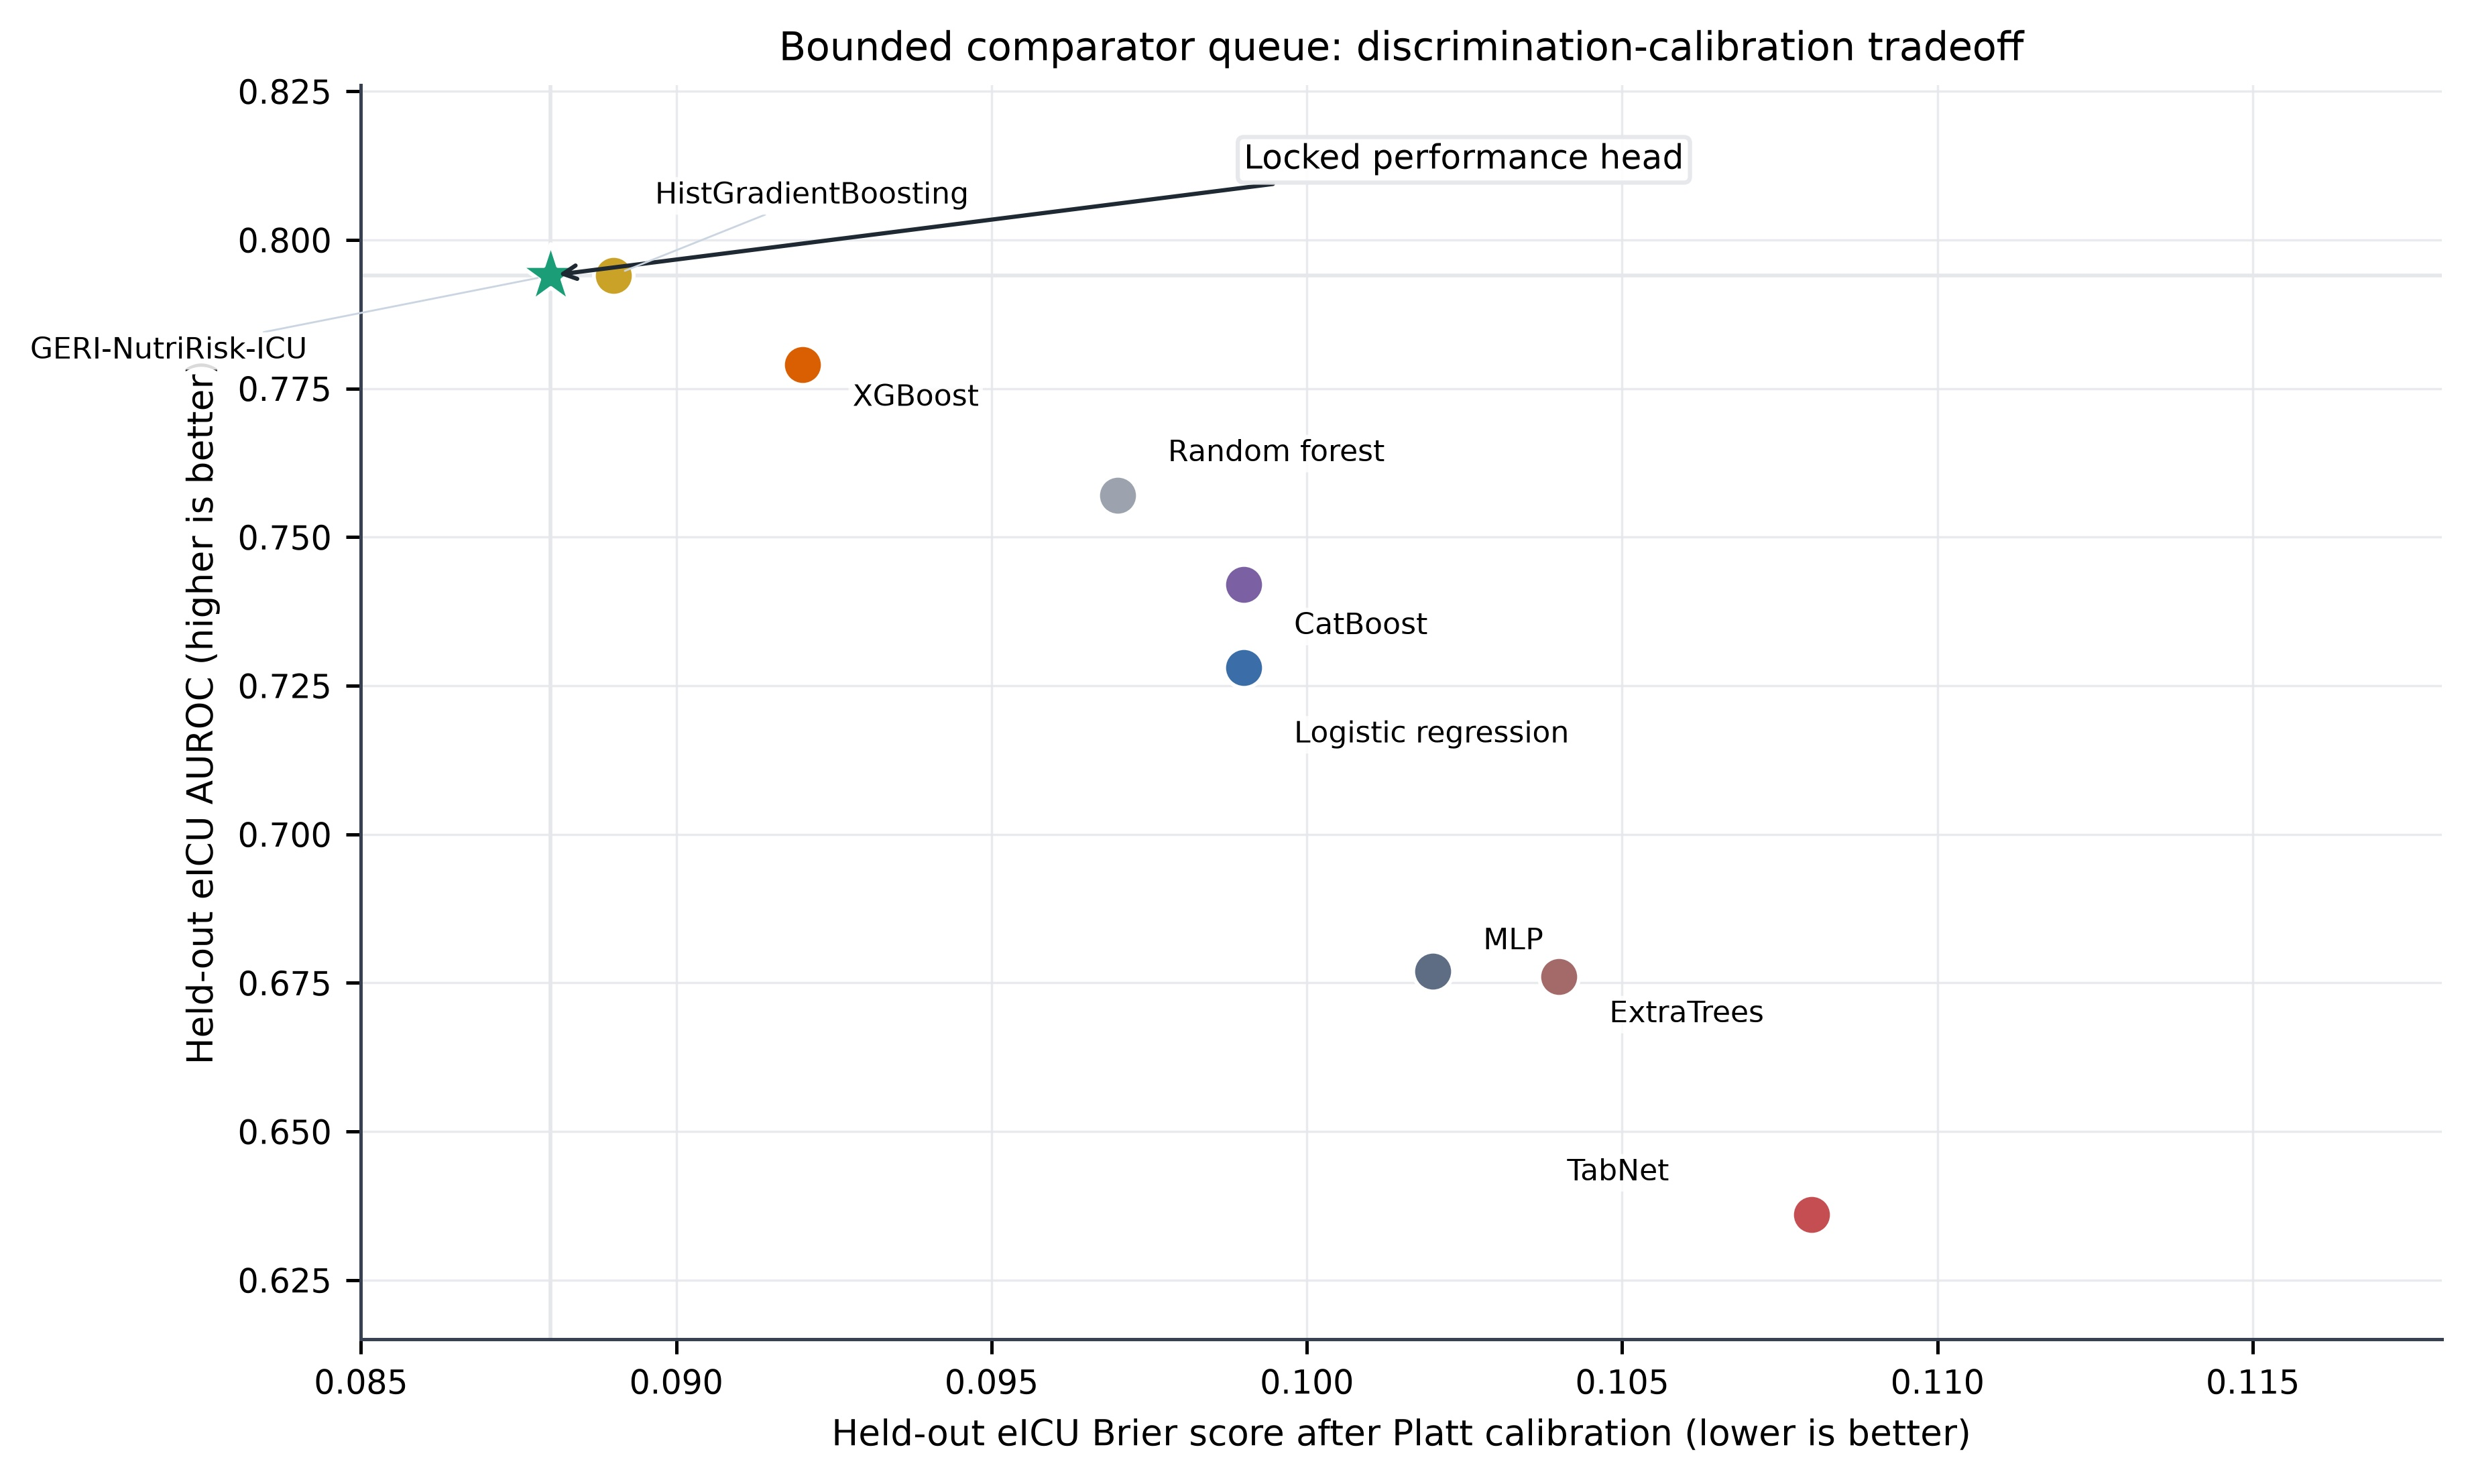
\includegraphics[width=0.90\textwidth]{../../figures/main_fig4_sota_completion_model_lock.jpg}
\caption{Bounded SOTA completion and model-lock analysis supporting LightGBM as the final performance head.}
\label{fig:sota_lock}
\end{figure}

\subsection{Locked Domain-Updated Performance}
After the model-lock step, the final GERI-NutriRisk-ICU framework used LightGBM as the performance head and logistic regression as the transparent interpretation anchor. The harmonized schema was expanded to 83 cross-database early-window variables and evaluated through a nested domain-update design: MIMIC-IV development data and a prespecified eICU local-update subset were used for model fitting, a disjoint eICU subset was used for Platt calibration, and the remaining eICU records were held out for final evaluation. In 57,488 held-out eICU stays, the locked model achieved AUROC 0.872, Brier score 0.073, and ECE 0.004 (Table~\ref{tab:v14_primary}). Compared with the 83-feature source-only plus Platt model, nested domain updating increased AUROC from 0.807 to 0.872 and reduced Brier score from 0.085 to 0.073. This gain identifies target-domain updating and disjoint calibration as central components of the final framework.

\begin{table}[htbp]
\centering
\caption{Locked GERI-NutriRisk-ICU V14 feature-set and nested domain-update performance in held-out eICU-CRD. Bold values indicate the best value in each displayed metric column; lower Brier score and ECE are better.}
\label{tab:v14_primary}
\resizebox{\textwidth}{!}{%
\begin{tabular}{llrrr}
\toprule
Feature set & Model & AUROC & Brier & ECE\\
\midrule
Full 83-feature schema (source-only + Platt) & GERI-NutriRisk-ICU & 0.807 & 0.085 & 0.014\\
w/o full nutrition construct & GERI-NutriRisk-ICU & 0.867 & 0.074 & \textbf{0.004}\\
w/o explicit nutrition variables & GERI-NutriRisk-ICU & 0.870 & 0.074 & 0.005\\
w/o nutrition-support indicators & GERI-NutriRisk-ICU & \textbf{0.873} & \textbf{0.073} & \textbf{0.004}\\
w/o nutrition/metabolic laboratories & GERI-NutriRisk-ICU & 0.866 & 0.074 & \textbf{0.004}\\
Full 83-feature schema (domain-updated) & GERI-NutriRisk-ICU & 0.872 & \textbf{0.073} & \textbf{0.004}\\
\bottomrule
\end{tabular}}
\end{table}

\subsection{APACHE-IV/IVa Same-Subset Benchmark}
The APACHE-IV/IVa benchmark placed the locked framework against established ICU severity comparators on the same evaluation records. APACHE-IV and APACHE-IVa predicted hospital mortality were available for 39,920 held-out eICU stays, and these predictions served as comparators rather than model inputs. On this identical subset, GERI-NutriRisk-ICU exceeded both APACHE versions in discrimination and Brier score (Table~\ref{tab:apache}). Against APACHE-IVa, GERI-NutriRisk-ICU achieved AUROC 0.871 versus 0.850, with paired AUROC difference 0.0209 (95\% CI 0.0158--0.0260), and Brier score 0.074 versus 0.082. The result shows that the locally updated, nutrition-aware harmonized framework added measurable predictive resolution beyond an APACHE-style global severity comparator while preserving calibrated absolute-risk estimates.

\begin{table}[htbp]
\centering
\caption{Same-subset comparison of APACHE-IV/IVa with GERI-NutriRisk-ICU in held-out eICU-CRD. Bold values indicate the better model value or the positive paired difference; lower Brier score is better.}
\label{tab:apache}
\resizebox{\textwidth}{!}{%
\begin{tabular}{lrrrrr}
\toprule
Comparator & Comparator AUROC & Comparator Brier & GERI-NutriRisk-ICU AUROC & GERI-NutriRisk-ICU Brier & AUROC difference (95\% CI)\\
\midrule
APACHE-IV & 0.846 & 0.085 & \textbf{0.871} & \textbf{0.074} & \textbf{0.0252} (0.0201--0.0305)\\
APACHE-IVa & 0.850 & 0.082 & \textbf{0.871} & \textbf{0.074} & \textbf{0.0209} (0.0158--0.0260)\\
\bottomrule
\end{tabular}}
\end{table}

\subsection{Nutrition-Feature Incremental Value in the Locked Model}
Nutrition-related variables showed their clearest contribution in the locked domain-updated model. In source-only MIMIC-to-eICU transport, full-minus-reduced contrasts were negative for several nutrition definitions, indicating that source-trained nutrition effects were sensitive to cross-database coding and measurement differences. After local domain updating and disjoint calibration, the direction reversed for the broader nutrition construct and for nutrition/metabolic laboratories (Table~\ref{tab:v14_nutrition}). Removing all nutrition-construct variables reduced AUROC by 0.0049 (95\% CI 0.0029--0.0071) and increased Brier score by 0.0011; removing nutrition/metabolic laboratories reduced AUROC by 0.0059 (0.0041--0.0077) and increased Brier score by 0.0012. Early nutrition-support indicators alone produced no stable incremental discrimination, which suggests that treatment-process indicators were less portable than measured metabolic and vulnerability markers. The combined pattern supports a modest, reproducible nutrition-related increment within the full ICU risk framework.

\begin{table}[htbp]
\centering
\caption{Paired nutrition-feature incremental value for GERI-NutriRisk-ICU in held-out eICU-CRD. Positive AUROC differences favor the full feature set; negative Brier differences favor the full feature set. Bold values indicate the largest favorable domain-updated contrast.}
\label{tab:v14_nutrition}
\resizebox{\textwidth}{!}{%
\begin{tabular}{lrrrr}
\toprule
Contrast & Source-only AUROC diff & Source-only Brier diff & Domain-updated AUROC diff & Domain-updated Brier diff\\
\midrule
Full minus w/o full nutrition construct & -0.0184 & 0.0027 & 0.0049 & -0.0011\\
Full minus w/o explicit nutrition variables & -0.0101 & 0.0021 & 0.0017 & -0.0007\\
Full minus w/o nutrition-support indicators & -0.0006 & 0.0002 & -0.0005 & -0.0001\\
Full minus w/o nutrition/metabolic laboratories & -0.0141 & 0.0024 & \textbf{0.0059} & \textbf{-0.0012}\\
\bottomrule
\end{tabular}}
\end{table}

\subsection{Explainability and Hospital-Cluster Robustness}
The locked V14 explanation analysis connected model performance to clinically interpretable feature domains. Permuting organ support and neurologic severity produced the largest loss of held-out discrimination (AUROC decrease 0.0627), followed by vital signs (0.0482), blood gas/perfusion variables (0.0199), and nutrition/metabolic laboratories (0.0160) (Figure~\ref{fig:importance}, Table~\ref{tab:importance}). This ordering is clinically informative: the model first organizes risk around acute organ dysfunction and physiologic instability, then refines risk using perfusion, chemistry, and nutrition/metabolic information. Leading gain-ranked features included Glasgow Coma Scale, calcium, blood urea nitrogen, respiratory rate, urine output, lactate, heart rate, cardiac ICU type, pH, and body mass index (Supplementary Figure S7). The presence of both severity variables and nutrition/metabolic variables among the leading predictors is consistent with the framework's design as an integrated geriatric ICU nutrition-risk stratifier.

\begin{figure}[htbp]
\centering
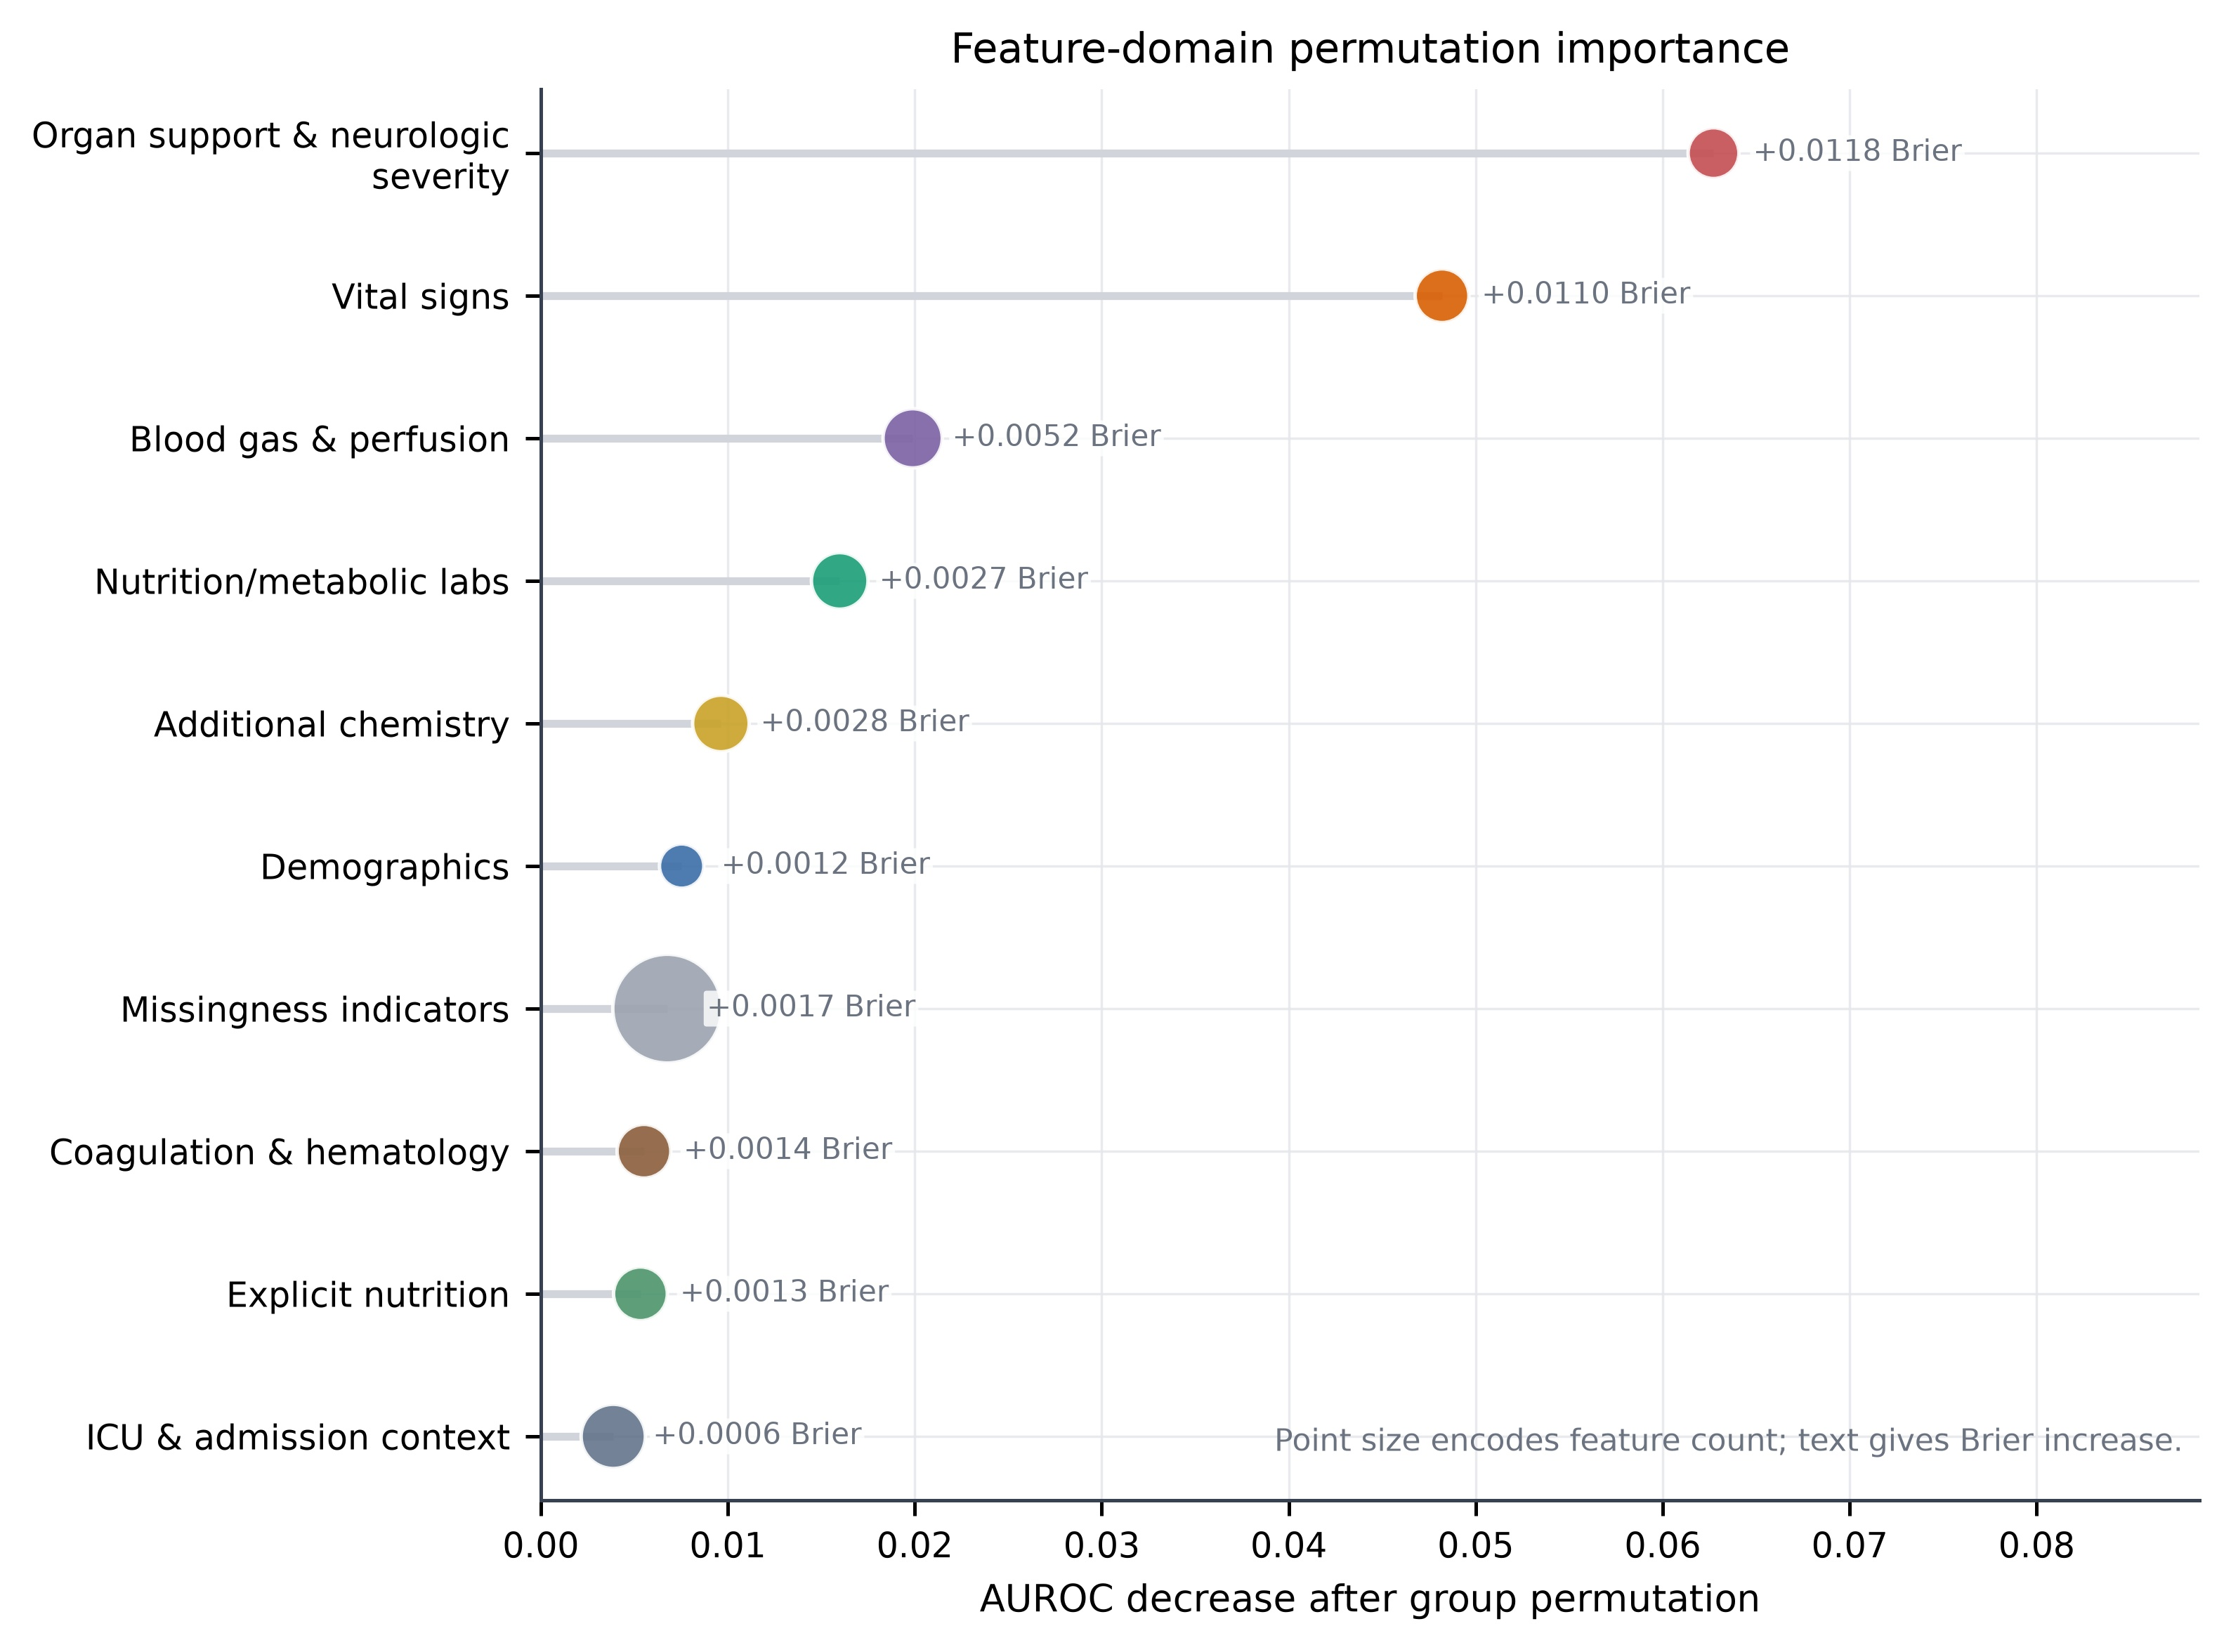
\includegraphics[width=0.76\textwidth]{../../figures/main_fig5_group_permutation_importance.jpg}
\caption{Feature-domain permutation importance for the locked domain-updated GERI-NutriRisk-ICU model.}
\label{fig:importance}
\end{figure}

\begin{table}[htbp]
\centering
\caption{Top feature domains by held-out AUROC decrease after grouped permutation. Bold values indicate the largest AUROC decrease.}
\label{tab:importance}
\begin{tabular}{lrr}
\toprule
Feature domain & Features & AUROC decrease\\
\midrule
Nutrition/metabolic laboratories & 6 & 0.0160\\
Additional chemistry & 6 & 0.0096\\
Blood gas and perfusion & 7 & 0.0199\\
Vital signs & 5 & 0.0482\\
Organ support and neurologic severity & 4 & \textbf{0.0627}\\
\bottomrule
\end{tabular}
\end{table}

Hospital-level analyses tested the distribution of performance across eICU sites. Across 206 held-out hospitals, AUROC remained 0.870 after excluding the ten largest hospitals, 0.874 among hospitals with at least 100 held-out stays, and 0.875 among hospitals with at least 200 held-out stays (Table~\ref{tab:hospital}). The small change across these restrictions indicates that performance was distributed across hospital-size strata. Hospital-cluster bootstrap further confirmed the APACHE-IVa comparison, with model-minus-APACHE-IVa AUROC mean 0.021 and 95\% cluster CI 0.015--0.028. Figure~\ref{fig:hospital} shows the hospital-level AUROC distribution, supporting the interpretation that the locked framework retained discrimination across multicenter eICU practice environments.

\begin{table}[htbp]
\centering
\caption{Hospital-cluster robustness for GERI-NutriRisk-ICU in held-out eICU-CRD. Bold values indicate the best displayed robustness metric; lower Brier score is better.}
\label{tab:hospital}
\begin{tabular}{lrrrr}
\toprule
Analysis subset & N & Events & AUROC & Brier\\
\midrule
All held-out hospitals & 57,488 & 7,130 & 0.872 & 0.073\\
Excluding top 10 hospitals by N & 44,777 & 5,330 & 0.870 & \textbf{0.072}\\
Hospitals with N $\geq$ 100 & 54,833 & 6,804 & 0.874 & 0.073\\
Hospitals with N $\geq$ 200 & 47,517 & 5,967 & \textbf{0.875} & 0.073\\
\bottomrule
\end{tabular}
\end{table}

\begin{figure}[htbp]
\centering
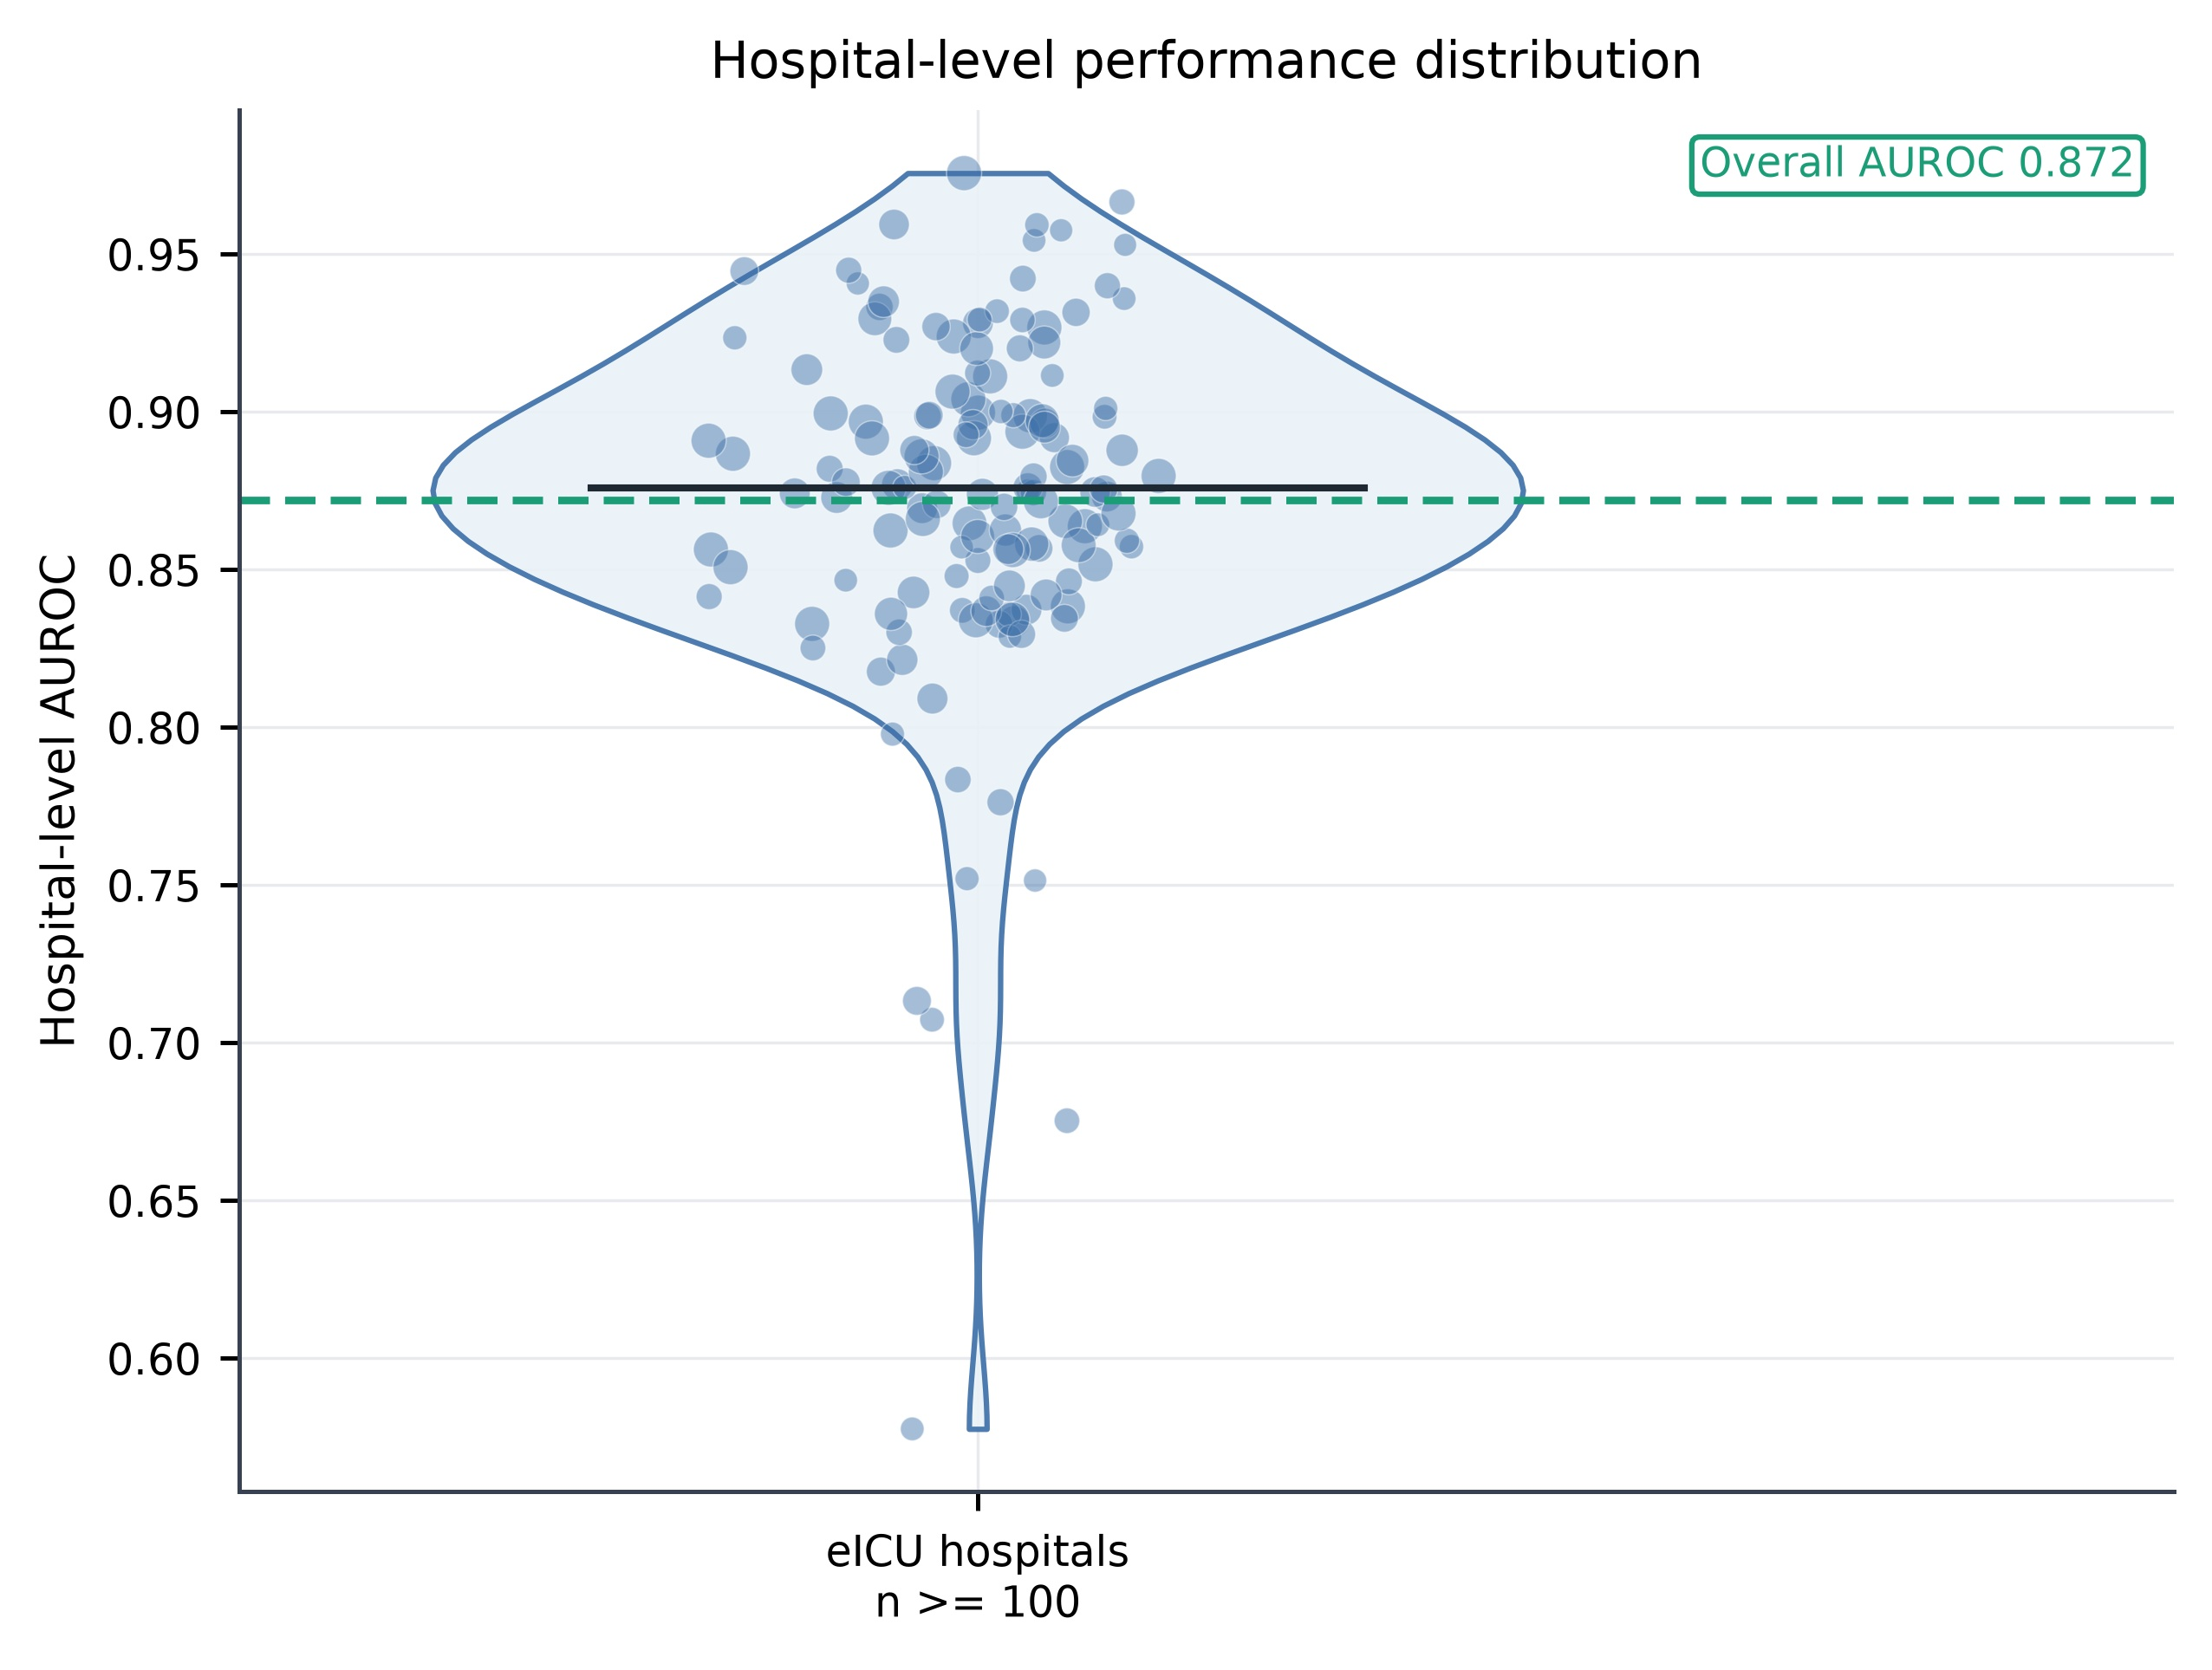
\includegraphics[width=0.72\textwidth]{../../figures/main_fig6_hospital_auc_distribution.jpg}
\caption{Hospital-level AUROC distribution among eICU hospitals with at least 100 held-out stays.}
\label{fig:hospital}
\end{figure}

\section{Discussion}

This study developed and externally evaluated GERI-NutriRisk-ICU, a nutrition-aware mortality-risk framework for older ICU patients. The main finding is not simply that a flexible tabular model achieved a high AUROC. Rather, the evidence chain shows that a harmonized geriatric ICU feature space, when paired with prespecified target-domain updating and disjoint calibration, can produce APACHE-contextualized mortality-risk stratification that remains interpretable and stable across a multicenter external database. This distinction is important for nutrition-facing critical-care prediction studies, because nutrition variables are highly entangled with acute severity, ordering practices, organ support, and database-specific documentation. A model that ignores this context can easily convert nutrition markers into weak stand-alone associations. GERI-NutriRisk-ICU instead evaluates nutrition-related variables inside a full severity framework and then tests the resulting predictions against APACHE-IV/IVa, calibration metrics, decision-curve evidence, feature-domain attribution, and hospital-cluster robustness.

\subsection{Principal Interpretation}
The APACHE comparison provides the clearest interpretation of the framework's added value. APACHE-IV and APACHE-IVa remain strong mortality-risk standards in ICU cohorts because they summarize acute physiology, chronic health status, diagnosis, and early treatment context \citep{Zimmerman2006ApacheIV}. In this study, the source-only MIMIC-trained models improved after feature expansion but did not exceed APACHE-IV/IVa in the APACHE-available eICU subset. That result establishes an important baseline: direct database transport is insufficient when the target database has different hospitals, workflows, coding conventions, and missingness structures. After local domain updating and independent calibration, however, the locked GERI-NutriRisk-ICU head achieved AUROC 0.871 versus 0.850 for APACHE-IVa on identical held-out records, with a paired AUROC difference of 0.0209 and a lower Brier score. The gain is moderate in absolute size, but it is clinically and methodologically meaningful because it is measured against a mature severity comparator on the same patients rather than against a weak statistical baseline.

This pattern also defines the intended use of the framework. GERI-NutriRisk-ICU should be read as a reproducible update-and-calibrate framework for older ICU populations, not as a fixed source-domain score ready for unmodified deployment in every hospital. The separation of development, local updating, calibration, and held-out evaluation follows contemporary prediction-model guidance, which emphasizes that external validation and model updating are distinct analytical steps \citep{Collins2024EvalPart1,Riley2024EvalPart2,Collins2024TRIPODAI}. Within that design, the disjoint calibration set protects the final held-out estimate from using the same records for both probability correction and evaluation. The low expected calibration error in the final eICU held-out cohort therefore strengthens the claim that the model does more than rank patients; it also returns risk probabilities that are better aligned with observed outcome frequencies.

\subsection{Nutrition-Related Signal}
The nutrition findings refine how nutrition information should be interpreted in older ICU risk stratification. Critical-care nutrition guidelines emphasize early recognition of nutritional vulnerability, but routinely available electronic variables rarely isolate malnutrition, intake adequacy, or response to nutrition therapy by themselves \citep{Singer2023ESPENPractical,Compher2022ASPEN,Compher2025GLIMCriticalIllness}. The present ablation results reflect that clinical reality. Removing nutrition-support indicators alone did not reduce discrimination, indicating that feeding-route documentation and early support decisions are insufficient as isolated predictive markers. In contrast, removing the broader nutrition construct and removing nutrition/metabolic laboratories reduced domain-updated AUROC by 0.0049 and 0.0059, respectively, with accompanying Brier-score improvements for the full model. These paired comparisons show that nutrition-related information contributes measurable incremental value when it is integrated with organ support, vital signs, blood gas/perfusion variables, and admission context.

The explainability results support the same interpretation. Organ support and neurologic severity produced the largest grouped permutation loss, followed by vital signs and blood gas/perfusion variables, confirming that the dominant risk structure remains acute critical illness. Nutrition/metabolic laboratories nevertheless ranked above several contextual and missingness domains, and individual gain rankings included blood urea nitrogen and body mass index. The result is therefore not a mechanistic claim that a single nutrition intervention changes mortality. It is a clinically coherent prediction claim: nutrition-related and metabolic variables help resolve residual heterogeneity among older ICU patients after major severity signals are already represented. This framing aligns the model with geriatric critical-care biology, where nutritional reserve, catabolism, renal-metabolic stress, frailty, and acute organ dysfunction jointly shape short-term vulnerability.

\subsection{External Validity, Robustness, and Clinical Utility}
The eICU design gives the external evaluation practical relevance because the target database includes many hospitals with heterogeneous case mix and documentation practices \citep{Pollard2018EICU}. Aggregate performance alone can hide concentration of benefit in a few large centers. The hospital-level analyses address this concern by showing stable discrimination after excluding the ten largest hospitals and after restricting evaluation to hospitals with at least 100 or 200 held-out stays. The hospital-cluster bootstrap also retained a positive AUROC difference versus APACHE-IVa. These results indicate that the model's APACHE-contextualized advantage was distributed across hospital strata rather than being driven entirely by high-volume sites.

Clinical utility depends on more than AUROC. A risk stratifier used for nutrition-aware surveillance must separate high-risk patients, keep probability estimates calibrated, and provide usable decision thresholds. The decision-curve analysis indicates net-benefit advantages across clinically plausible thresholds, while calibration metrics show that local updating and Platt recalibration improved probability alignment. These properties matter because nutritional assessment and escalation are workflow-sensitive: an overconfident model can increase unnecessary consults and interventions, whereas an under-calibrated model can miss older patients whose vulnerability is not fully captured by diagnosis or organ-support variables. GERI-NutriRisk-ICU is therefore best positioned as a decision-support layer for prospective risk surveillance, enrichment of nutrition-assessment workflows, and audit of high-risk geriatric ICU subgroups.

\subsection{Limitations and Future Work}
Several limitations define the boundary of these findings. First, the study is retrospective and depends on database-specific recording, measurement frequency, coding practice, and missingness mechanisms. Harmonization across MIMIC-IV and eICU-CRD reduces this problem but cannot make the two databases identical. Second, the outcome is in-hospital mortality. This endpoint is auditable and clinically important, but it is not a direct measure of malnutrition status, nutrition adequacy, muscle mass, feeding tolerance, functional recovery, or treatment response. Third, the APACHE-superior result applies to the nested domain-updated and calibrated framework, not to source-only MIMIC-to-eICU transport. In practical terms, implementation at a new institution should include local data auditing, mapping checks, recalibration, and prospective silent-mode monitoring before clinical use.

Fourth, nutrition-related variables were derived from routinely available structured data. They capture body size, metabolic laboratories, selected treatment processes, and missingness patterns, but they do not contain detailed caloric or protein delivery, dietitian assessments, indirect calorimetry, body-composition imaging, or longitudinal nutrition trajectories. Fifth, the bounded model queue reduced post hoc model shopping and included conventional machine-learning and neural tabular comparators, but it did not exhaust all possible tabular foundation models, feature-engineering variants, or hyperparameter spaces. Finally, hospital-cluster robustness strengthens multicenter external validity but does not replace prospective implementation validation. Future work should test GERI-NutriRisk-ICU in prospective workflows, evaluate whether calibrated risk strata improve nutrition-assessment prioritization, and determine whether nutrition-aware surveillance changes process measures and patient-centered outcomes.

\section{Conclusion}

GERI-NutriRisk-ICU provides a reproducible framework for early mortality-risk stratification in older ICU patients that is externally evaluated, locally updateable, calibrated, APACHE-contextualized, and nutrition-aware. Across harmonized MIMIC-IV and eICU-CRD cohorts, the locked domain-updated model outperformed APACHE-IV/IVa on identical held-out eICU records, retained stable performance across hospital strata, and showed that nutrition/metabolic variables add modest but reproducible predictive value within an integrated severity model. These findings support prospective evaluation of GERI-NutriRisk-ICU as a nutrition-aware surveillance layer for geriatric critical care.

\section*{Conflict of Interest Statement}
The authors declare that the research was conducted in the absence of any commercial or financial relationships that could be construed as a potential conflict of interest.

\section*{Author Contributions}
ZJ: Conceptualization, Methodology, Software, Formal analysis, Writing - original draft. HS: Methodology, Validation, Data curation, Writing - review \& editing. YZ: Software, Benchmark curation, Visualization, Reproducibility audit. SW: Supervision, Resources, Project administration, Writing - review \& editing.

\section*{Funding}
The authors declare that no financial support was received for the research, authorship, and/or publication of this article.

\section*{Acknowledgments}
The authors acknowledge the PhysioNet, MIMIC-IV, and eICU-CRD teams for maintaining credentialed access to de-identified critical-care research databases.

\section*{Data Availability Statement}
The patient-level data analyzed in this study are available to credentialed users through PhysioNet after completion of the required training and data-use agreements: MIMIC-IV v3.1, \url{https://physionet.org/content/mimiciv/3.1/} and \url{https://doi.org/10.13026/kpb9-mt58}; and eICU Collaborative Research Database v2.0, \url{https://physionet.org/content/eicu-crd/2.0/} and \url{https://doi.org/10.13026/C2WM1R}. Patient-level records cannot be redistributed by the authors. Aggregate result tables, figure source data, and non-identifying reproducibility materials are available in the public code repository at \url{https://github.com/Hajimi-Sudo/geri-nutririsk-icu}.

\section*{Code Availability Statement}
The analysis scripts, manuscript figure/table export scripts, aggregate result tables, and reproducibility manifests are available at \url{https://github.com/Hajimi-Sudo/geri-nutririsk-icu}. The repository does not contain patient-level MIMIC-IV or eICU-CRD records, derived patient-level feature tables, or credentialed database files.

\section*{Ethics Statement}
This secondary analysis used de-identified critical-care databases available through PhysioNet. The authors accessed and analyzed the data after completing the required credentialing and data-use agreements. No direct patient contact or re-identification was performed.

\bibliographystyle{Frontiers-Vancouver}
\bibliography{references}

\end{document}
